\IEEEPARstart{H}{abiendo} ya realizado detalladamente el an\'alsis propuesto
por la metdolog\'ia explicada en la secci\'on~\ref{subsec:metodologia} para
el caso de \emph{c\'amara fija, im\'agen fija} (secci\'on
\ref{subsec:fija-fija}), no ahondaremos tanto en detalles sobre la explicaci\'on
de los datos obtenidos. Los gr\'aficos, tablas e histogramas utilizados son los
mismos para este caso y los que le siguen\footnote{C\'amara m\'ovil, im\'agen
fija y m\'ovil.}. Simplemente expondremos los resultados y los analizaremos.

%---------------------------------------------------------------
\subsubsection{Spline}

\begin{figure}[H]
    \centering
    \subfloat[][ECM para 1 frames interpolados]{
        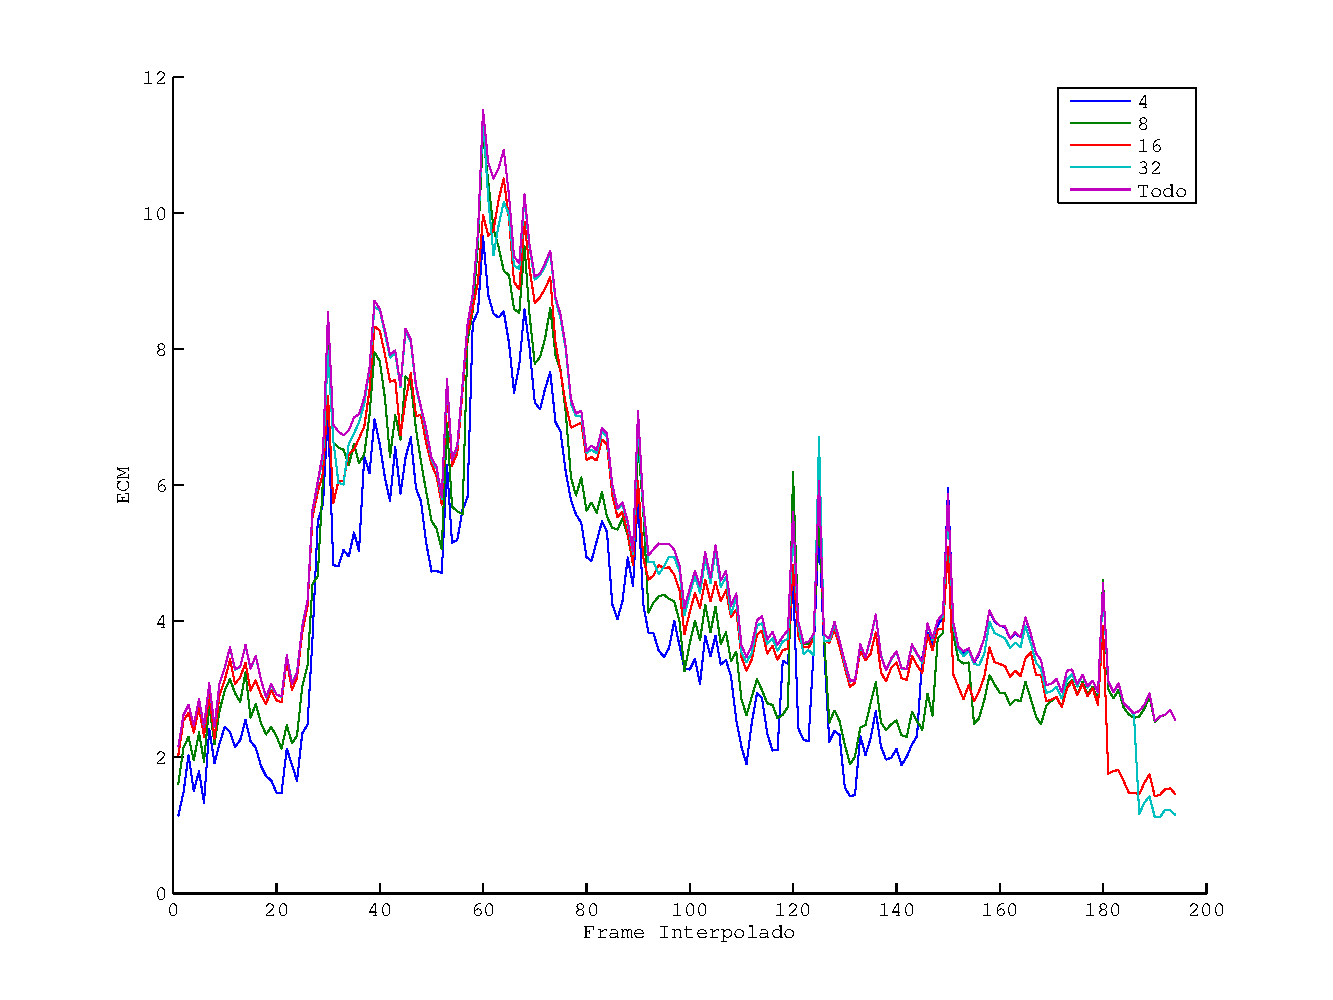
\includegraphics[width=.5\textwidth]{mse_spline-camara_fija-imagen_movil-k1.pdf}
        \label{subfig:fija-movil_spline-mse-k1}
    }
    \subfloat[][ECM para 10 frames interpolados]{
        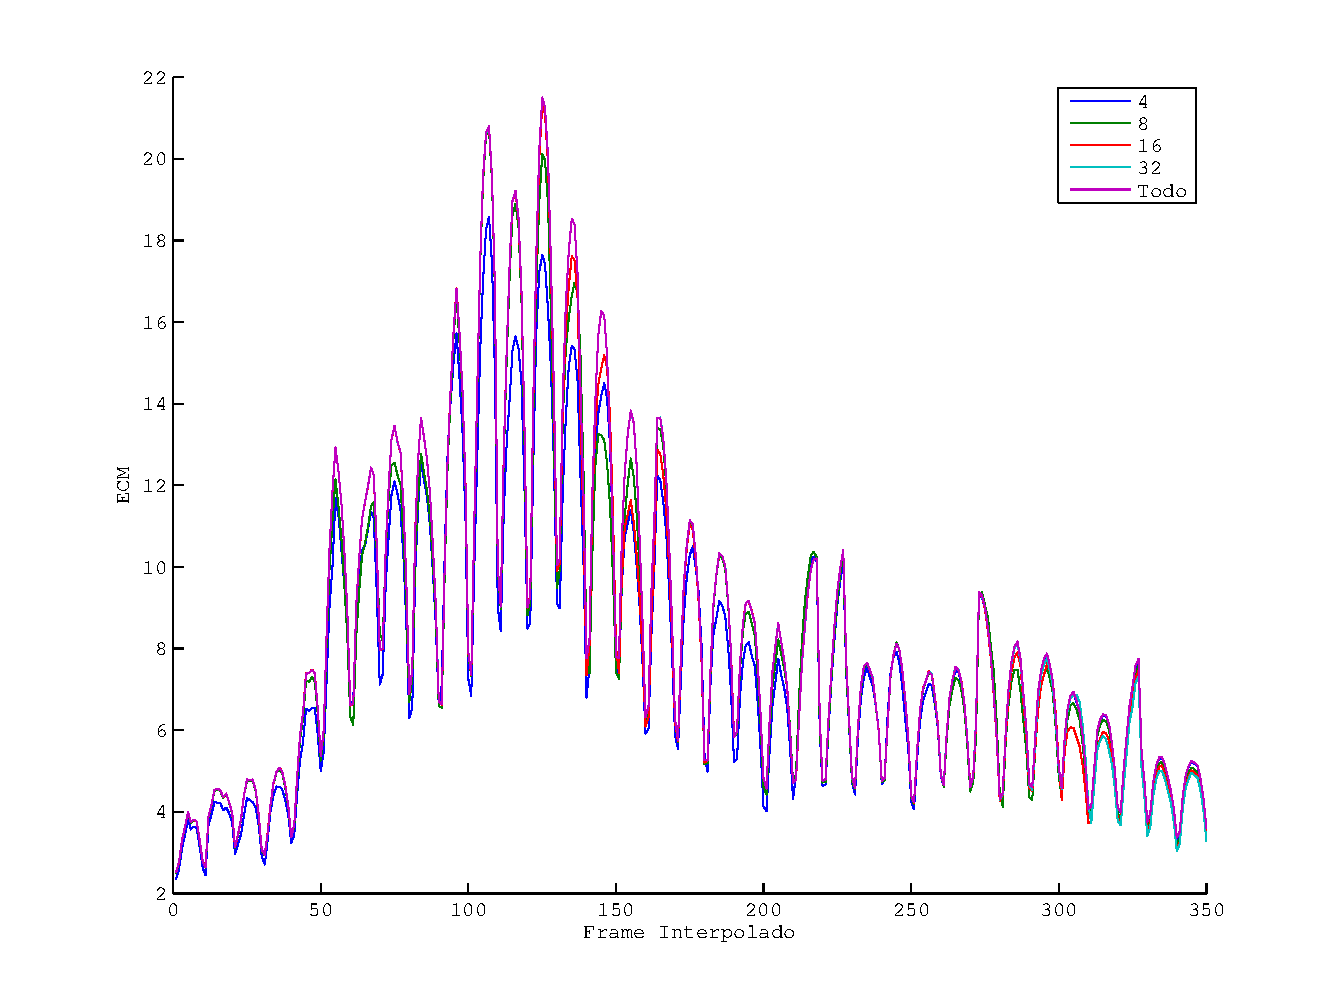
\includegraphics[width=.5\textwidth]{mse_spline-camara_fija-imagen_movil-k10.pdf}
        \label{subfig:fija-movil_spline-mse-k10}
    }\\
    \subfloat[][PSNR para 1 frames interpolados]{
        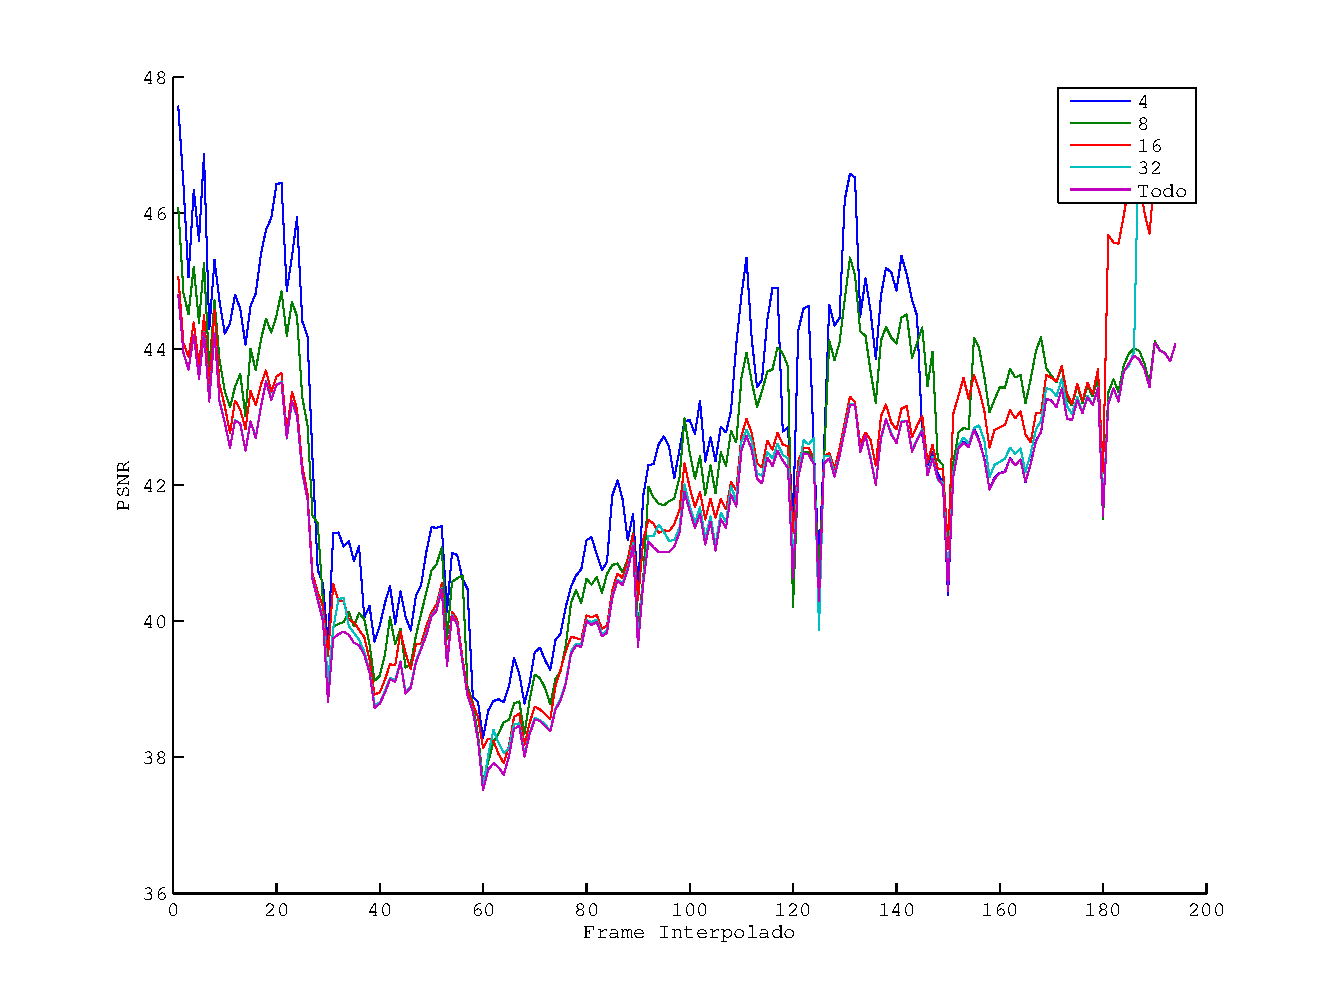
\includegraphics[width=.5\textwidth]{psnr_spline-camara_fija-imagen_movil-k1.pdf}
        \label{subfig:fija-movil_spline-psnr-k1}
    }
    \subfloat[][PSNR para 10 frames interpolados]{
        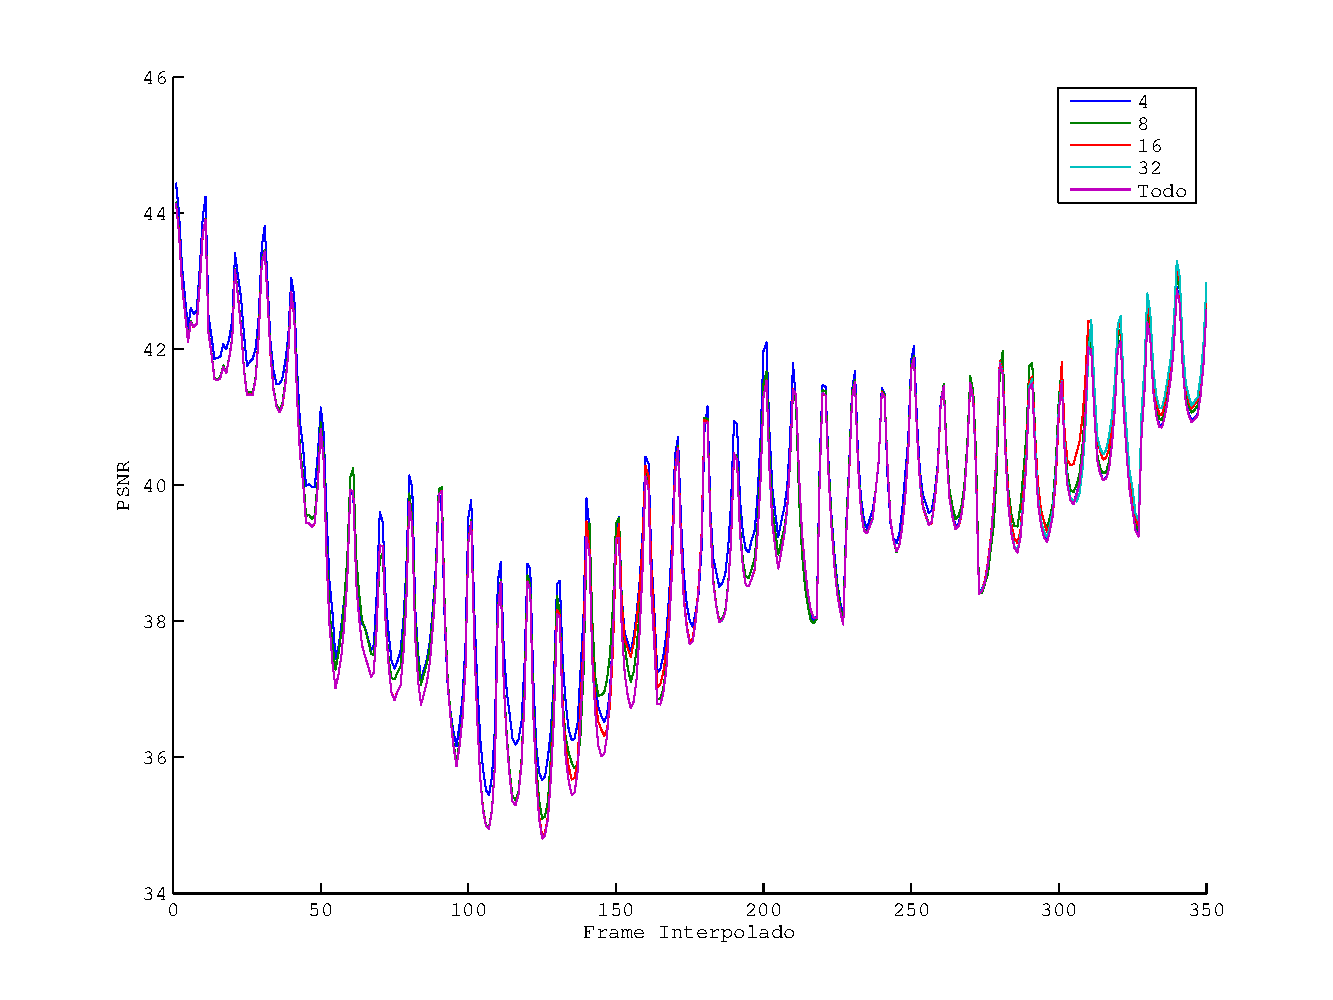
\includegraphics[width=.5\textwidth]{psnr_spline-camara_fija-imagen_movil-k10.pdf}
        \label{subfig:fija-movil_spline-psnr-k10}
    }
    \caption{Comparativa tama\~no de bloque para 1 y 10 frames interpolados}
    \label{fig:fija-movil_spline-mse-bloques}
\end{figure}

\par En primer lugar, al igual que para el experimento previo, se exponen
s\'olo los gr\'aficos comparativos de tama\~no de bloque del ECM por frame para
1 y 10 frames interpolados (figura \ref{fig:fija-movil_spline-mse-bloques}). No
se exponen los casos para 2 y 5 frames interpolados ya que el comportamiento
observado se refleja de la misma manera en estos, y para explicar el mismo
alcanza con las variantes expuestas.

\par Lo que se observa inicialmente de la figura
\ref{subfig:fija-movil_spline-mse-k1} respecto del tama\~no de bloque, es que
para este video el tama\~no de bloque 4 pareciera ser significativamente
mejor\footnote{Menos error.} que para los dem\'as tama\~nos (m\'as all\'a de
algunos pocos frames donde esto no ocurre). M\'as a\'un, en t\'erminos generales
m\'as all\'a de frames excepcionales, se observa que el ECM aumenta a medida que
aumenta el tama\~no de bloque.

\par Sin embargo, esto no pareciera ser tan claro para el caso de 10 frames
interpolados (figura \ref{subfig:fija-movil_spline-mse-k10}). En \'este se puede
distinguir que el tama\~no de bloque 4 suele tener menos error que el resto de
los tama\~nos, aunque la diferencia es notoriamente menor que para el caso de
1 frame interpolado. Y, \'aun m\'as, no queda claro a simple vista que el error
vaya aumentando a medida que aumenta el tama\~no de bloque (solapamiento de los
ECM), aunque s\'i podemos afirmar que la interpolaci\'on por spline para todo
el video (sin dividir en bloques) es el que suele tener para la gran mayor\'ia
de los frames el ECM m\'as alto. Este solapamiento no queda del todo claro en
esta figura, principalmente dado que la escala difiere respecto de la figura
\ref{subfig:fija-movil_spline-mse-k1}, pero queda ya claro al observar los
gr\'aficos de PSNR, que tienen la particularidad de normalizar respecto del
valor m\'aximo de los p\'ixeles los valores del ECM.

\par M\'as a\'un, si tenemos en cuenta el ECM/PSNR para 2 y 5 frames interpolados,
el patr\'on que se observa es que a medida que se interpolan m\'as frames se
incrementa el solapamiento, es decir, se ''pegan'' las funciones de ECM para
los distintos tama\~nos de bloque. Aunque, como parte de este patr\'on, pareciera
que a menor tama\~no de bloque se sigue comientiendo menos error.

\par B\'asicamente, se observa un patr\'on: a menor tama\~no de bloque menor
error cometido, aunque esta diferencia a favor de una interpolaci\'on de menor
tama\~no de bloque se va diluyendo a medida que se incrementa la cantidad de
frames interpolados.

\par Si nos detenemos en los cuadros de la figura
\ref{fig:fija-movil-dif_ecm_splines}, se observar\'a que se confirm\'a este
patr\'on\footnote{A modo de recordatorio, cada cuadro nos indica la diferencia
m\'axima del error para un mismo frame interpolado. B\'asicamente, en la
posici\'on $i,j$, tendremos la diferencia m\'axima de las estimaciones sobre
las cuales el tama\~no de bloque $i$ cometi\'o un error mayor que tama\~no
$j$.}. Se puede observar aqu\'i que para cualesquiera 2 tama\~nos de bloque
distintos, la m\'axima diferencia del ECM para un mismo frame siempre es mayor
para el tama\~no de bloque mayor. Por ejemplo, si tomamos los tama\~nos 4 y 8,
veremos que siempre 4 vs 8 (la diferencia m\'axima para la cual el ECM de 4 es
mayor al de 8) es mayor a 8 vs 4.

\begin{figure}[H]
    \centering
    \subfloat[][1 Frame Interpolado]{
        \footnotesize
        \setlength{\tabcolsep}{3pt}
        \begin{tabular}{|l|r|r|r|r|r|}
            \hline
            \textbf{Bloque}& \textbf{vs 4}& \textbf{vs 8}& \textbf{vs 16}& \textbf{vs 32}& \textbf{vs Entero}\\
            \hline\hline
            \textbf{4}&0& 1.0553& 1.3580& 1.5157& 0.0836\\
            \textbf{8}&2.2855& 0& 1.3654& 1.4776& 0.5794\\
            \textbf{16}&2.4014& 1.8014& 0& 0.3766& 0.0696\\
            \textbf{32}&2.5348& 1.8834& 1.4168& 0& 0.6421\\
            \textbf{Entero}&2.5429& 1.9027& 1.5443& 1.5157& 0\\
            \hline
        \end{tabular}
    }\hspace{10pt}
    \subfloat[][2 Frames Interpolados]{
        \footnotesize
        \setlength{\tabcolsep}{3pt}
        \begin{tabular}{|l|r|r|r|r|r|}
            \hline
            \textbf{Bloque}& \textbf{vs 4}& \textbf{vs 8}& \textbf{vs 16}& \textbf{vs 32}& \textbf{vs Entero}\\
            \hline\hline
            \textbf{4}&0& 1.0587& 1.4019& 1.5831& 0.5797\\
            \textbf{8}&2.6425& 0& 1.1953& 1.4636& 0.7106\\
            \textbf{16}&2.7262& 1.6141& 0& 0.3542& 0.0415\\
            \textbf{32}&2.7816& 1.7799& 1.3980& 0& 0.0566\\
            \textbf{Entero}&2.7875& 1.7952& 1.4049& 1.5831& 0\\
            \hline
        \end{tabular}
    }\\
    \subfloat[][5 Frames Interpolados]{
        \footnotesize
        \setlength{\tabcolsep}{3pt}
        \begin{tabular}{|l|r|r|r|r|r|}
            \hline
            \textbf{Bloque}& \textbf{vs 4}& \textbf{vs 8}& \textbf{vs 16}& \textbf{vs 32}& \textbf{vs Entero}\\
            \hline\hline
            \textbf{4}&0& 0.8709& 0.6384& 1.8067& 0.6342\\
            \textbf{8}&3.4411& 0& 0.6755& 1.6095& 0.6634\\
            \textbf{16}&3.5990& 3.2710& 0& 1.4143& 0.1297\\
            \textbf{32}&3.6145& 3.3025& 0.9938& 0& 0.0607\\
            \textbf{Entero}&3.6162& 3.3024& 1.0310& 1.8448& 0\\
            \hline
        \end{tabular}
    }\hspace{10pt}
    \subfloat[][10 Frames Interpolados]{
        \footnotesize
        \setlength{\tabcolsep}{3pt}
        \begin{tabular}{|l|r|r|r|r|r|}
            \hline
            \textbf{Bloque}& \textbf{vs 4}& \textbf{vs 8}& \textbf{vs 16}& \textbf{vs 32}& \textbf{vs Entero}\\
            \hline\hline
            \textbf{4}&0& 1.5891& 0.8529& 0.6327& 0.5407\\
            \textbf{8}&3.2999& 0& 1.5430& 0.7919& 0.7928\\
            \textbf{16}&3.6673& 2.3288& 0& 0.5000& 0.5016\\
            \textbf{32}&3.8571& 3.0513& 2.4365& 0& 0.2676\\
            \textbf{Entero}&3.8574& 3.0504& 2.4367& 0.6565& 0\\
            \hline
        \end{tabular}
    }
    \caption{Diferencia m\'axima de ECM para mismo frame seg\'un tama\~no de bloque}
    \label{fig:fija-movil-dif_ecm_splines}
\end{figure}


\par Ahora bien, siguiendo esta l\'inea de an\'alisis, se observa (salvo alguna
excepci\'on) otro patr\'on: a medida que se interpolan m\'as frames, las
diferencias m\'aximas del ECM incrementarse para los casos de tama\~no $i$ vs
$j$ con $i>j$, y decrementarse para $i<j$. Es decir, mientras que en el
gr\'afico \ref{subfig:fija-movil_spline-psnr-k10} se observa un mayor
solapamiento del PSNR, en las tablas de la figura
\ref{fig:fija-movil-dif_ecm_splines} vemos que las diferencias m\'aximas (o
picos) entre dos interpolaciones con distinto tama\~no de bloque se incrementan
a mayor cantidad de frames interpolados. Es decir, si bien en la media los
tama\~nos de bloque est\'an cada vez m\'as cerca a mayor cantidad de frames
interpolados, los errores m\'aximos cometidos por las interpolaciones con mayor
tama\~no de bloque respecto de los de menor tama\~no se incrementan (es decir,
mayores picos de error entre distintos tama\~nos\footnote{A no confundir con
los picos de error absoluto. Aqu\'i nos referimos a los errores m\'aximos entre
dos interpolaciones de la misma cantidad de frames pero distinto tama\~no se
incrementa a mayor cantidad de frames interpolados.}).

\begin{figure}[H]
    \centering
    \subfloat[][Valor Medio]{
        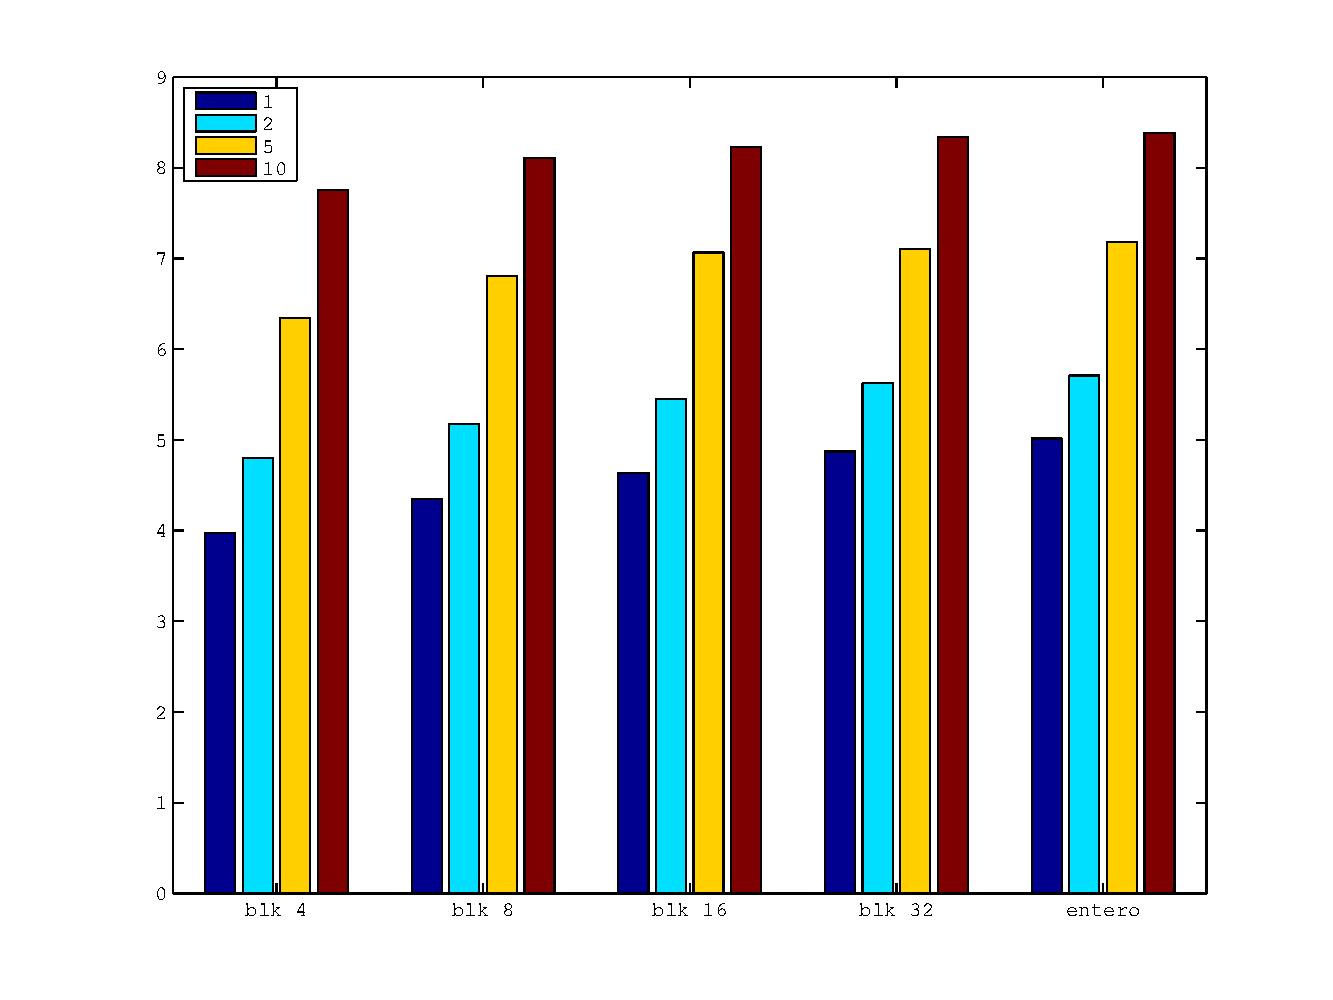
\includegraphics[width=.5\textwidth]{camara_fija-imagen_movil-mean_spline.pdf}
    }
    \subfloat[][Desv\'io Est\'andar]{
        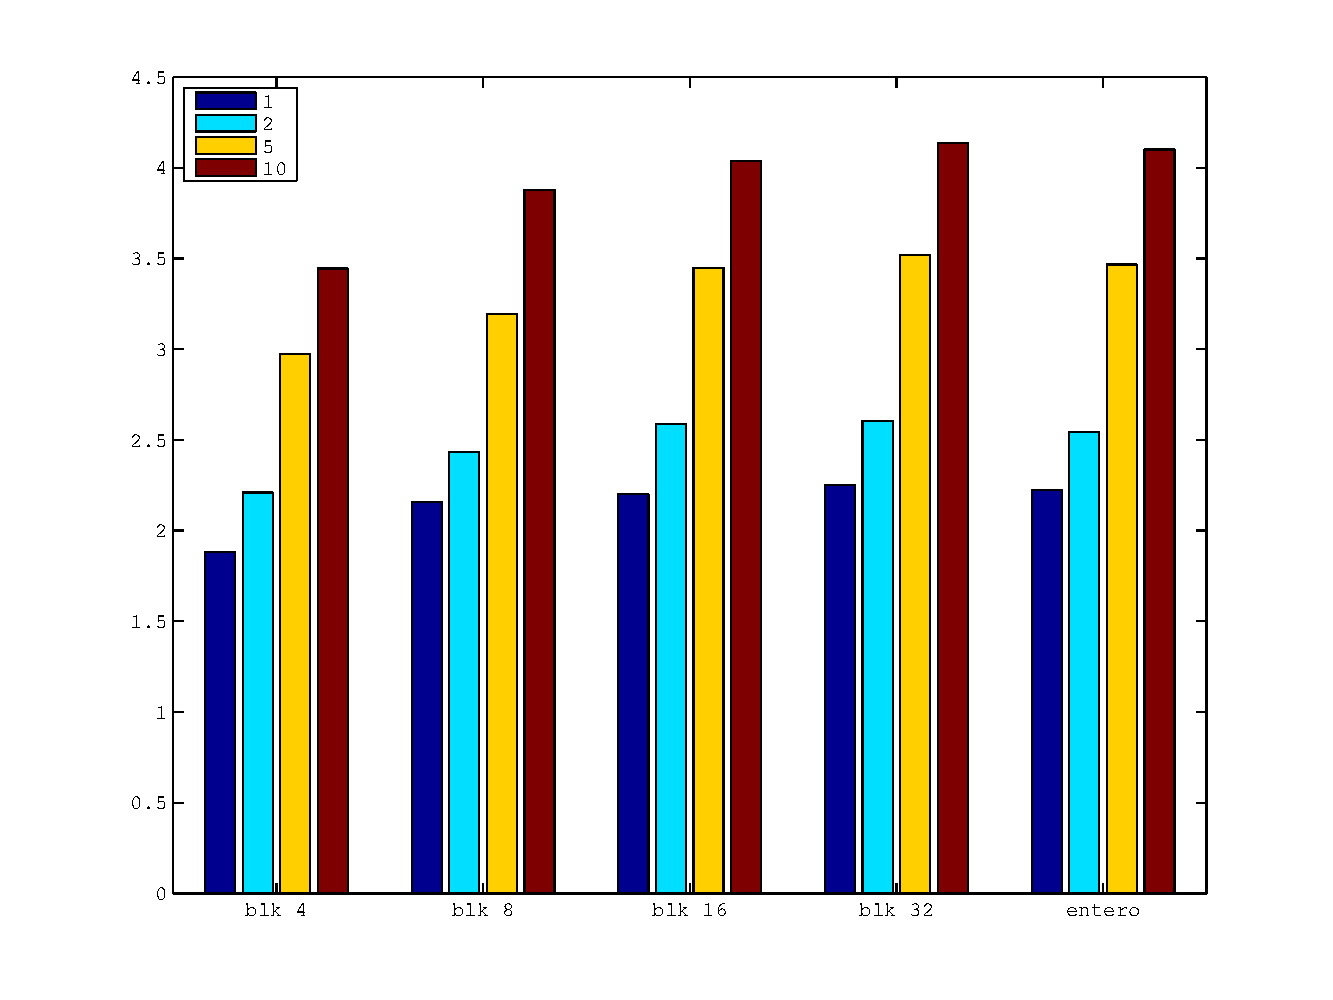
\includegraphics[width=.5\textwidth]{camara_fija-imagen_movil-std_spline.pdf}
    }\\
    \subfloat[][M\'aximo]{
        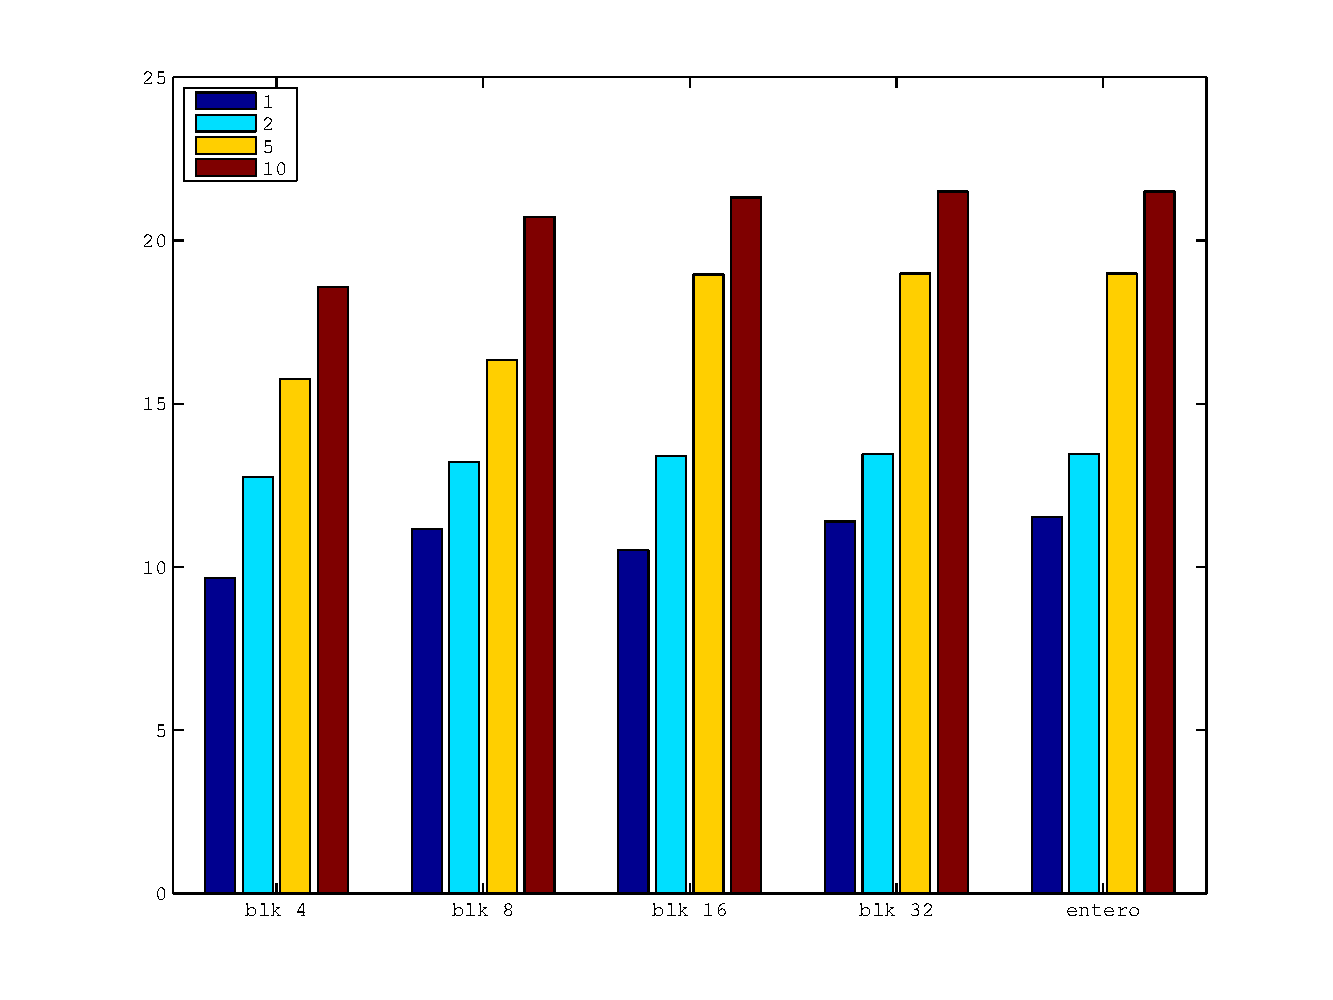
\includegraphics[width=.5\textwidth]{camara_fija-imagen_movil-max_spline.pdf}
    }
    \subfloat[][M\'inimo]{
        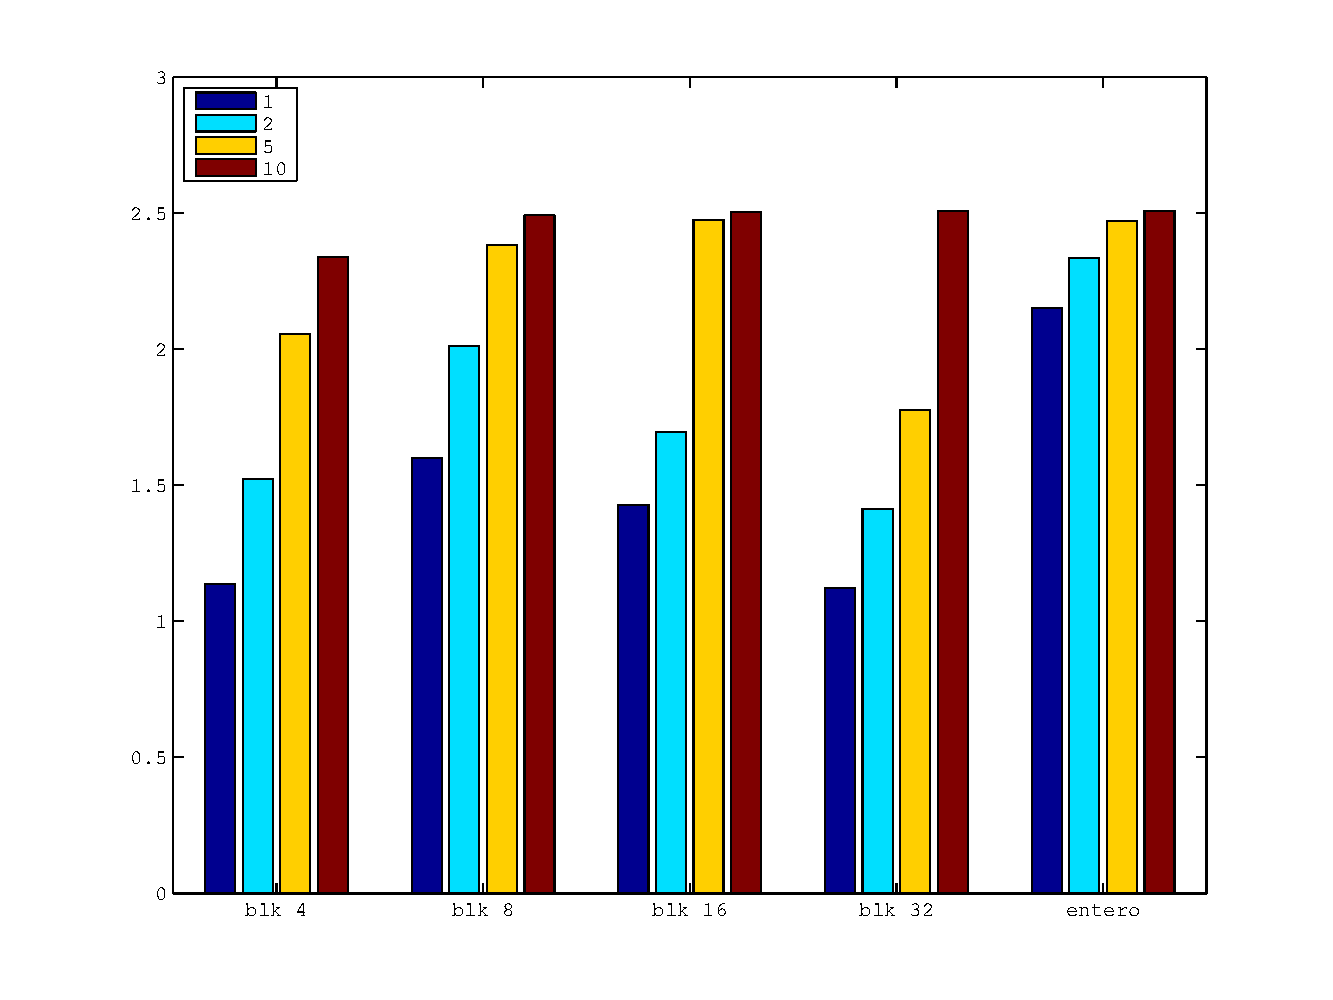
\includegraphics[width=.5\textwidth]{camara_fija-imagen_movil-min_spline.pdf}
    }
    \caption{Est\'adisticas ECM Seg\'un Frames Interpolados - Spline}
    \label{fig:fija-movil_spline-mse_estadisticas}
\end{figure}

\par En las estad\'isticas expuestas en la figura
\ref{fig:fija-movil_spline-mse_estadisticas} se observa otra confirmaci\'on del
patr\'on mencionado. Se puede ver que la media del ECM para una misma cantidad
de frames interpolados (barras del mismo color) es menor a menor tama\~no de
bloque (aunque las diferencias no son tan significativas entre tama\~nos
consecutivos). Y tambi\'en se observa que esta media es menor a menor cantidad
de frames interpolados, lo que es consistente con nuestras hip\'otesis
iniciales.

\par Tambi\'en observamos que este patr\'on se mantiene en el caso del desv\'io
est\'andar de los datos. Es decir, hay una varianza menor para a menor cantidad
de frames interpolados, y ligeramente menor para una misma cantidad de frames
interpolados pero con tama\~nos de bloque menores.

\par Otra cosa que destaca de la figura \ref{fig:fija-movil_spline-mse-bloques}
es que se observa una mayor cantidad de errores (o menor PSNR) en los primeros
frames (el primer cuarto de video). Analizando el video
comparativo\footnote{\url{https://drive.google.com/open?id=0B0RfkWV-4-XqSHJ3NXBSRUo4SjQ}}
de las diferencias entre frames originales e interpolados para tama\~no de
bloque 4 (menor ECM medio) y 10 frames interpolados (mayor varianza dentro de
las variantes de cantidad de frames interpolados)\footnote{La elecci\'on de
estos par\'ametros para le generaci\'on del video de diferencias frame a frame
se basa en los mismos argumentos que en el caso de splines del experimento
previo.}, observamos que al comienzo del video (una jugada de un partido de
f\'utbol desde un punto fijo) tenemos un jugador que comienza a correr en un
primer plano, mientras que el resto de los jugadores en movimiento se
encuentran en un plano cada vez m\'as lejano. En la figura
\ref{fig:fija-movil_spline-heatmap} se observa una captura del video comparador
representativo de esto.

\begin{figure}[H]
    \centering
    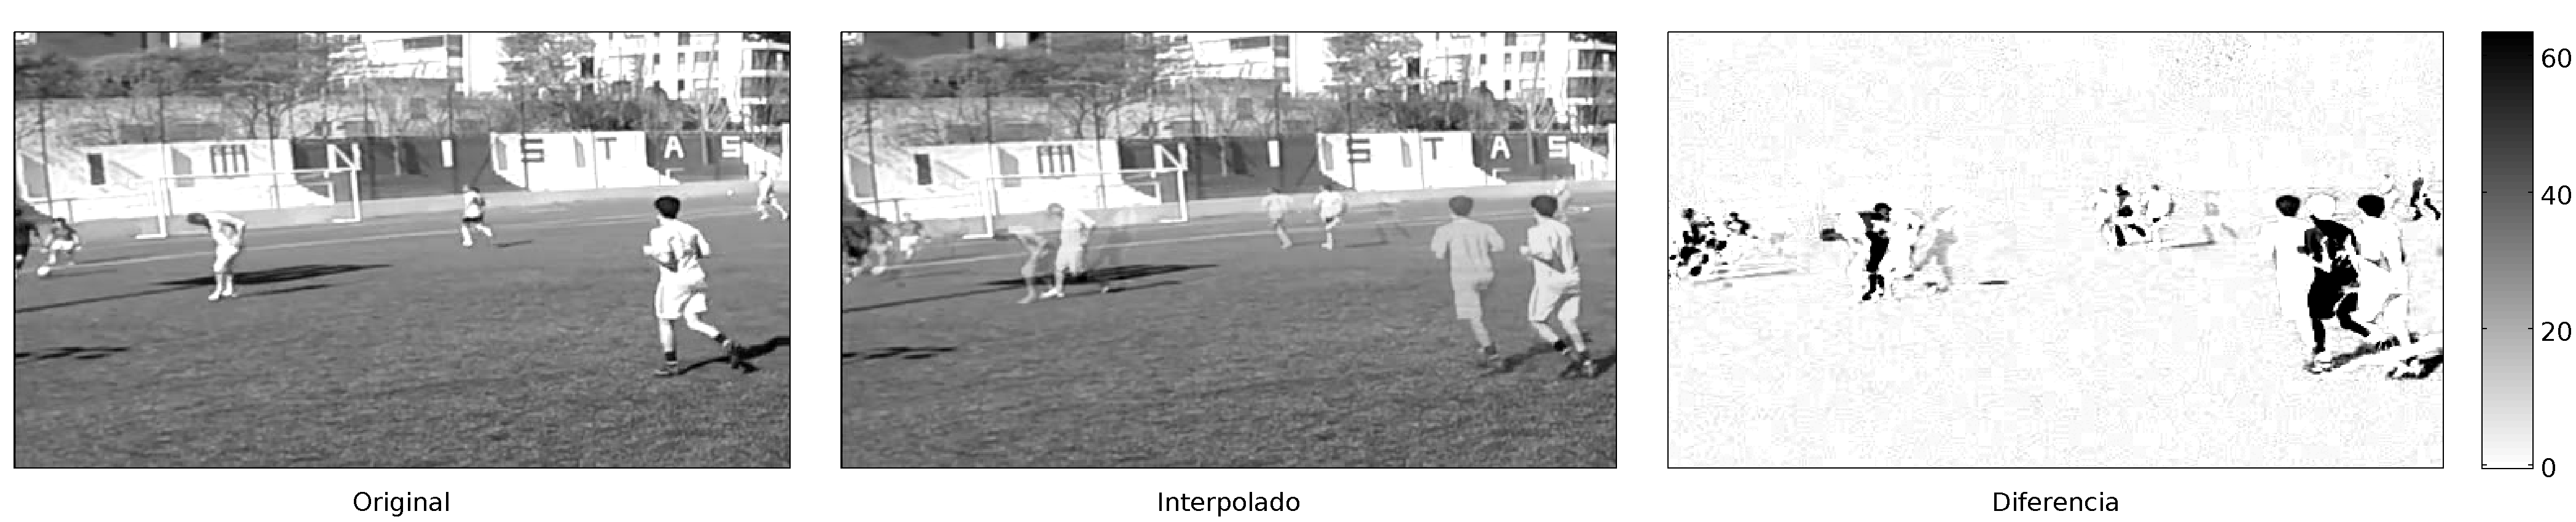
\includegraphics[width=\textwidth]{camara_fija-imagen_movil-spline-k10-blk4.png}
    \label{fig:fija-movil_spline-heatmap}
    \caption{Regi\'on peor aproximada por la interpolaci\'on por spline}
\end{figure}

\par En el video comparador queda claro que los movimientos de los jugadores
son los que m\'as error aportan a la interpolaci\'on. Y no s\'olo eso, sino que
el hecho de que haya jugadores en planos m\'as cercanos a la c\'amara generan
un mayor error en la interpolaci\'on, ya que dichos jugadores ''ocupan'' una
mayor cantidad de pixeles de los frames que aquellos que se encuentran en
planos m\'as lejanos. Este jugador que comienza en un plano m\'as cercano, al
comenzar a pasar a planos cada vez m\'as lejanos comienza a ser representado por
cada vez menos p\'ixeles, y as\'i entonces cada vez disminuye su injerencia
en el error de la interpolaci\'on (menos pixeles interpolados con cambios debidos
al desplazamiento de este jugador). Y esto queda evidenciado en las primeras
figuras donde observamos que en el \'ultimo cuarto de video/frames los picos del
ECM son menores (o que los del PSNR son cada vez mayores).

%---------------------------------------------------------------
\subsubsection{Interpolaci\'on Lineal}

\begin{figure}[H]
    \centering
    \subfloat[][Valor Medio]{
        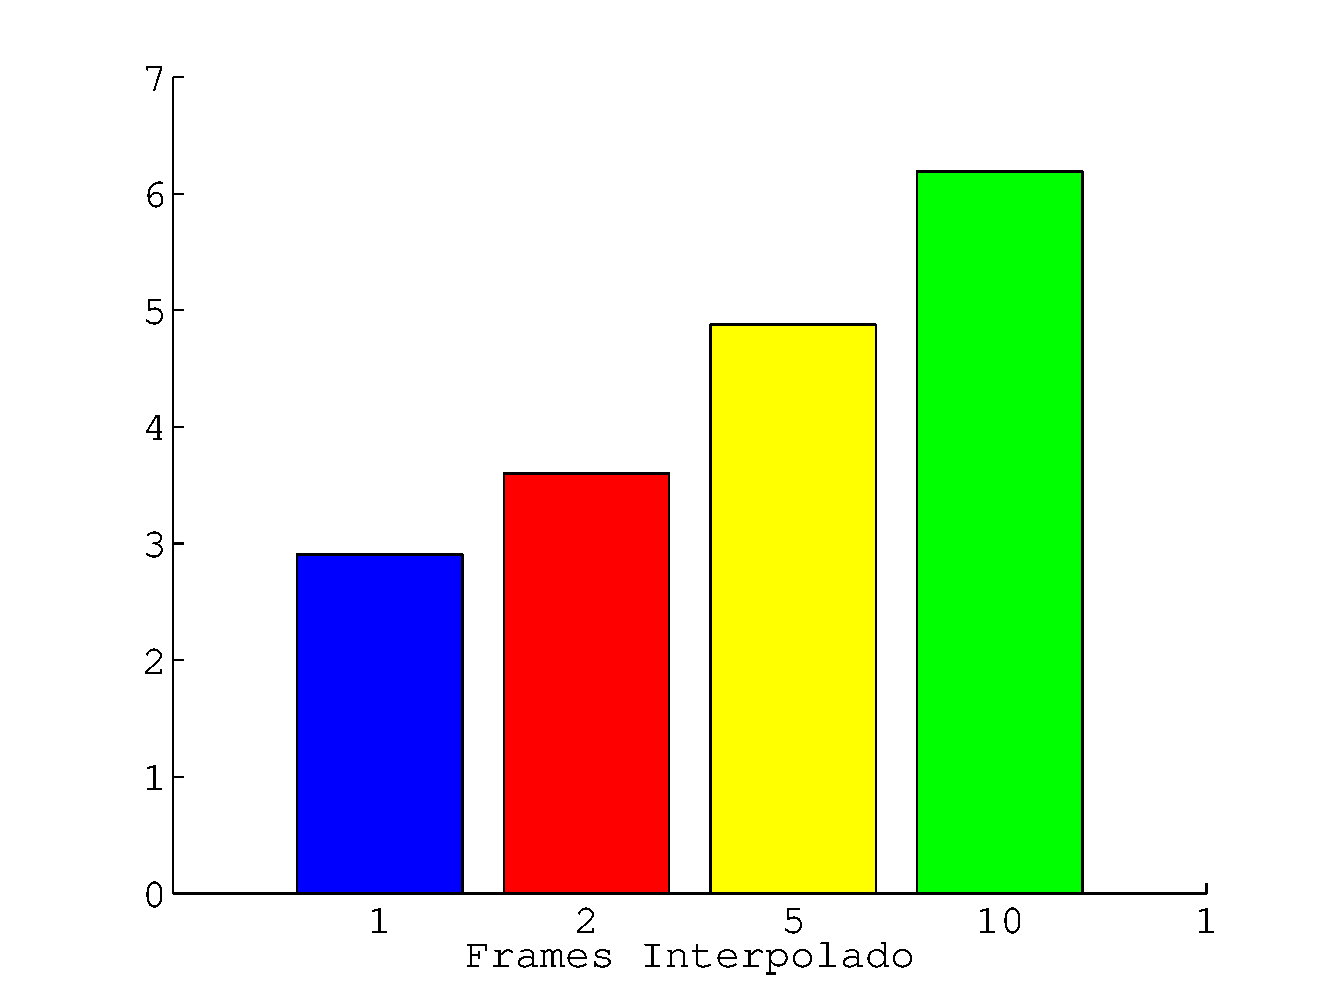
\includegraphics[width=.25\textwidth]{camara_fija-imagen_movil-mean_lineal.pdf}
    }
    \subfloat[][Desv\'io Est\'andar]{
        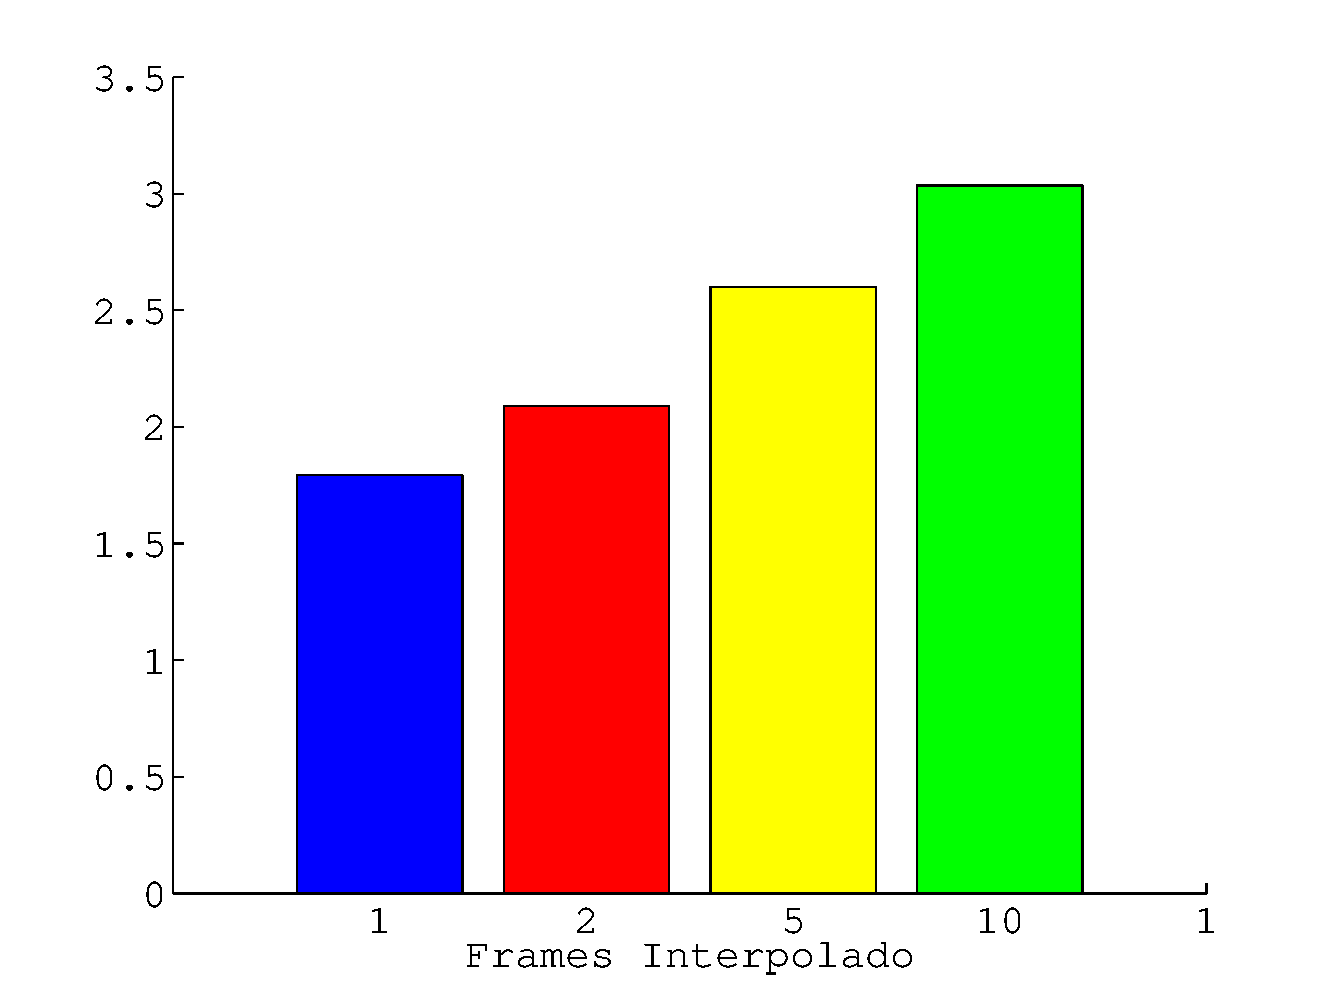
\includegraphics[width=.25\textwidth]{camara_fija-imagen_movil-std_lineal.pdf}
    }
    \subfloat[][M\'aximo]{
        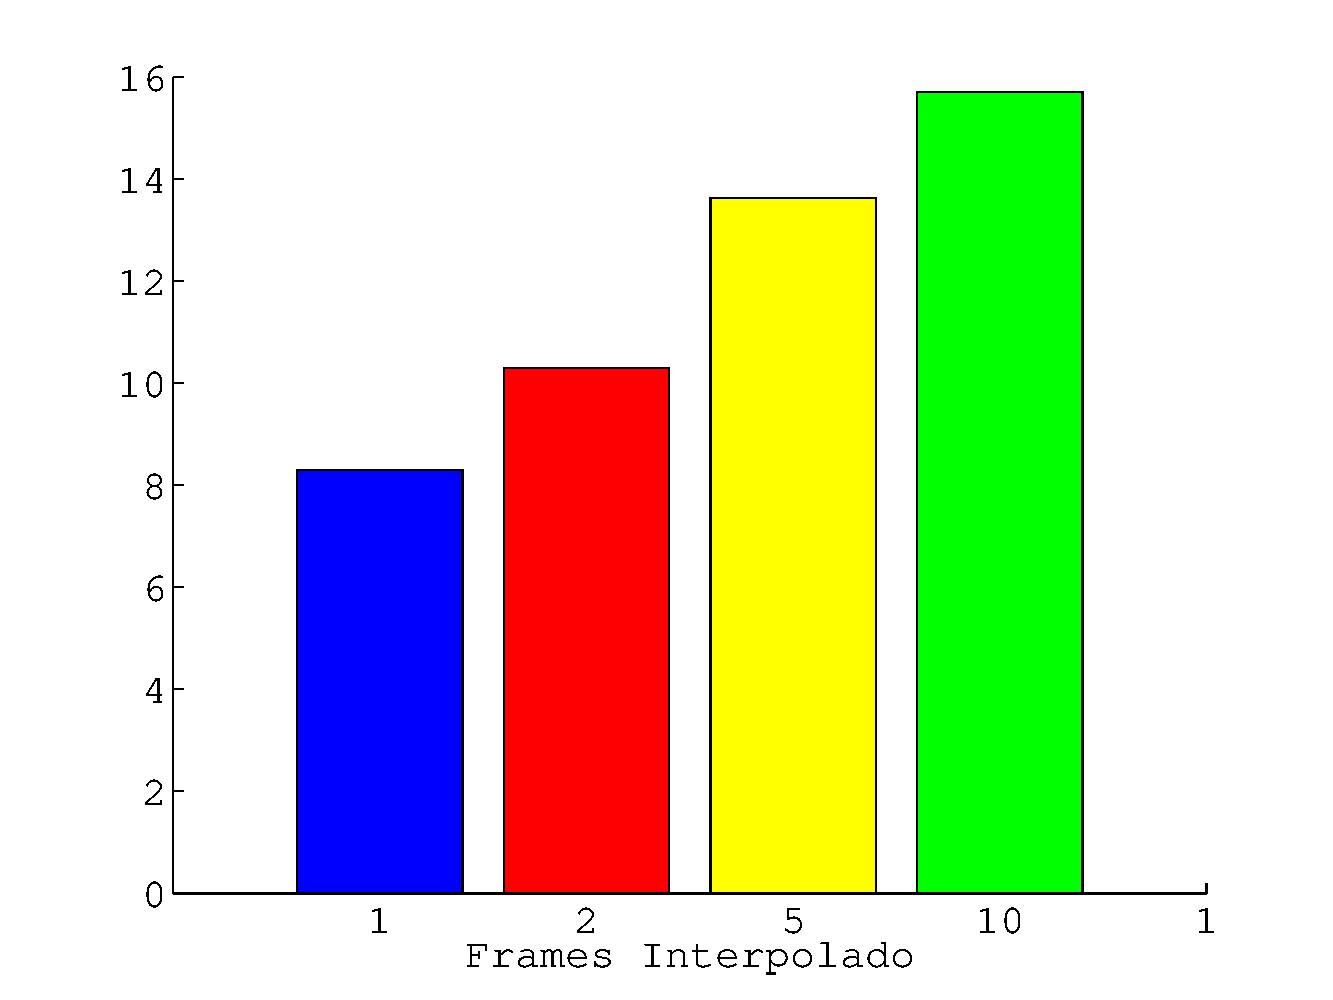
\includegraphics[width=.25\textwidth]{camara_fija-imagen_movil-max_lineal.pdf}
    }
    \subfloat[][M\'inimo]{
        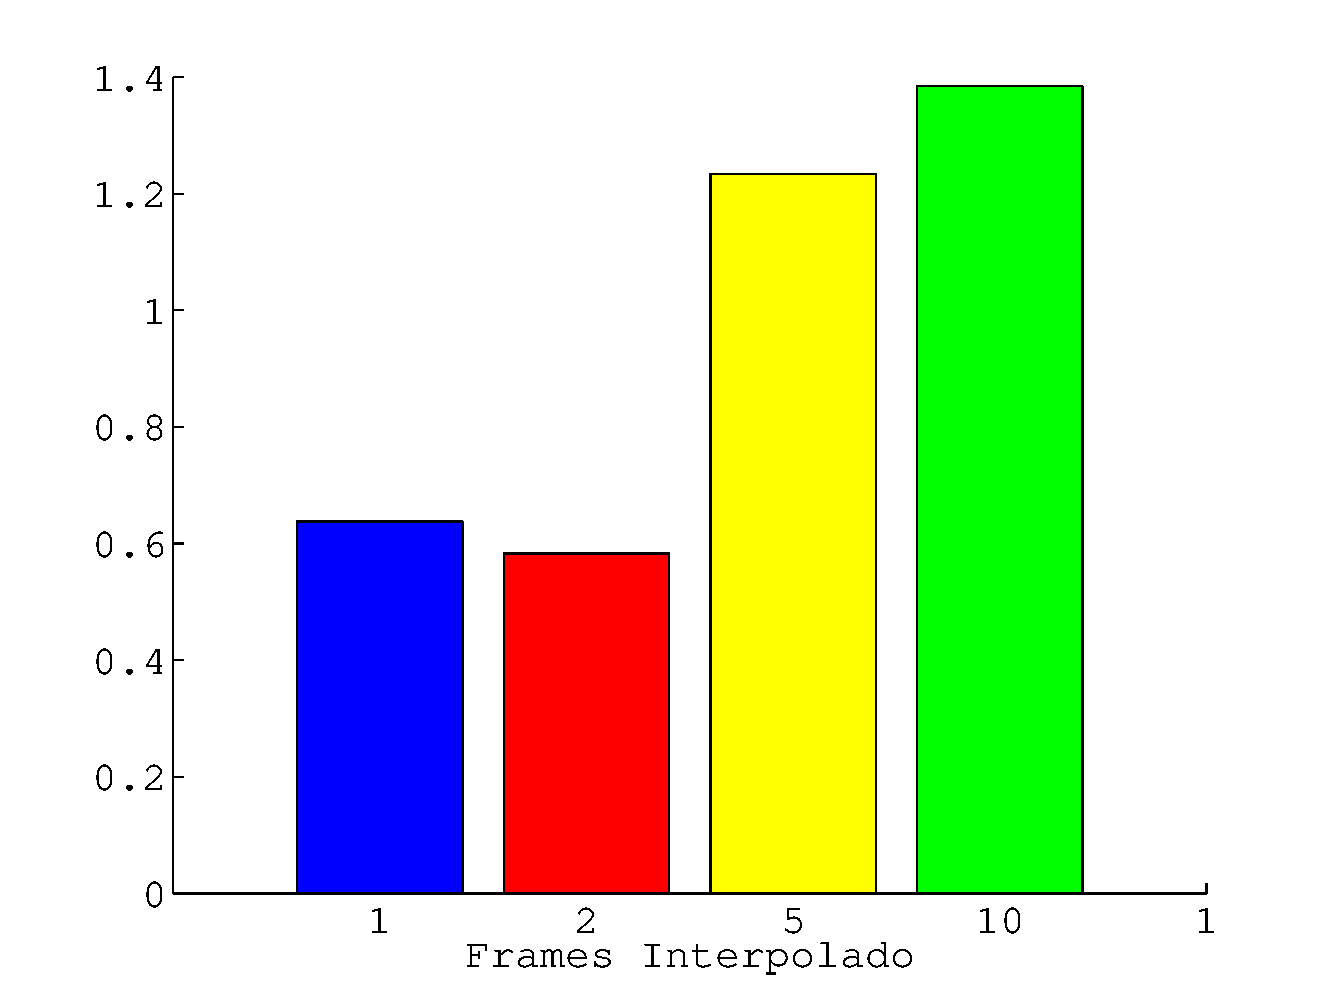
\includegraphics[width=.25\textwidth]{camara_fija-imagen_movil-min_lineal.pdf}
    }
    \caption{Est\'adisticas ECM Seg\'un Frames Interpolados - M\'etodo Lineal}
    \label{fig:fija-movil_lineal-mse_estadisticas}
\end{figure}

\par Observando las est\'adisticas del m\'etodo para las distintas variantes
de la cantidad de frames interpolados, se hayan resultados que son consistentes
con las hip\'otesis iniciales enunciadas. Se observa como el ECM medio es cada
vez mayor a medida que se interpolan m\'as frames (es decir, se utilizan 2 frames
para interpolar una cantidad cada vez mayor de frames entre ambos).

\par Adem\'as tambi\'en se observa que la varianza del error de la
aproximaci\'on de la interpolaci\'on aumenta conforme aumenta la cantidad de
frames interpolados (lo cual es de alguna manera razonable, al interpolarse
m\'as frames, los frames interpolados m\'as cercanos a los frames utilizados en
la interpolaci\'on tendr\'an menor error, mientras que a mayor distancia de
estos m\'as error habr\'a, generando multiples valores de error distintos y
distantes entre s\'i -y de la media-). Este \'ultimo comportamiento se puede
observar m\'as claramente en la figura \ref{fig:fija-movil_lineal-psnr-k10}.

\begin{figure}
    \centering
    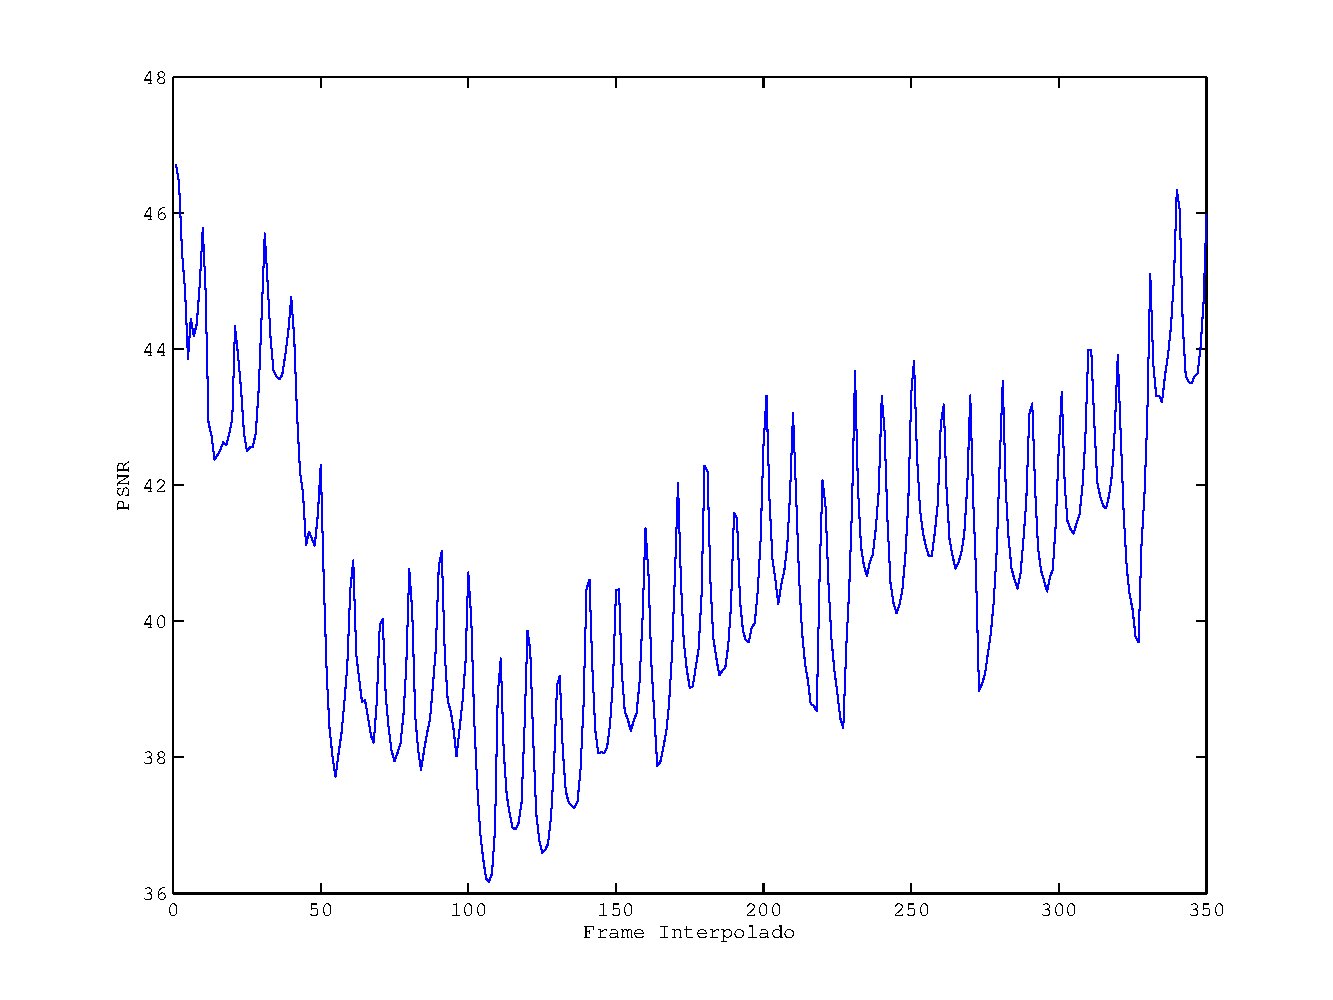
\includegraphics[width=.85\textwidth]{camara_fija-imagen_movil-lineal-psnr-k10.pdf}
    \caption{PSNR para 10 frames interpolados - M\'etodo Lineal}
    \label{fig:fija-movil_lineal-psnr-k10}
\end{figure}

\par Aqu\'i se puede observar como el PSNR\footnote{Recordemos que el PSNR, a
diferencia del ECM, nos da una noci\'on de la calidad de la estimaci\'on del
frame. Es decir, a mayor PSNR, menor ECM (aunque la relaci\'on no es lineal, ya
que el PSNR normaliza la medida seg\'un el valor m\'aximo de los p\'ixeles).}
tiene un comportamiento oscilante, yendo de un valor ''alto'' de PSNR a uno
bajo y luego comenzando a ascender nuevamente hasta llegar a otro pico ''alto''.

\par De la observaci\'on se determin\'o que estos picos ''altos'' son los frames
interpolados inmediatos a los frames originales utilizados para calclular la
funcion interpoladora, y no es coincidencia que los picos ''bajos'' (donde hay
mayor error en la interpolaci\'on) sean justamente los frames intermedios entre
dos frames utilizados para calcular el polinomio interpolador lineal.

\par Pasando a analizar el video comparador para 10 frames
interpolados\footnote{\url{https://drive.google.com/open?id=0B0RfkWV-4-XqMHNrY3JqVHlOUXc}},
observamos el mismo comportamiento visto para el caso de splines, aunque los
errores cometidos para las reginoes con poco (o ning\'un) movimiento
parecer\'ian ser menores que para splines. En todo caso, esto se estudiar\'a al
final de esta secci\'on al comparar los distintos m\'etodos entre s\'i.

%---------------------------------------------------------------
\subsubsection{Vecino m\'as Cercano}

\begin{figure}[H]
    \centering
    \subfloat[][Valor Medio]{
        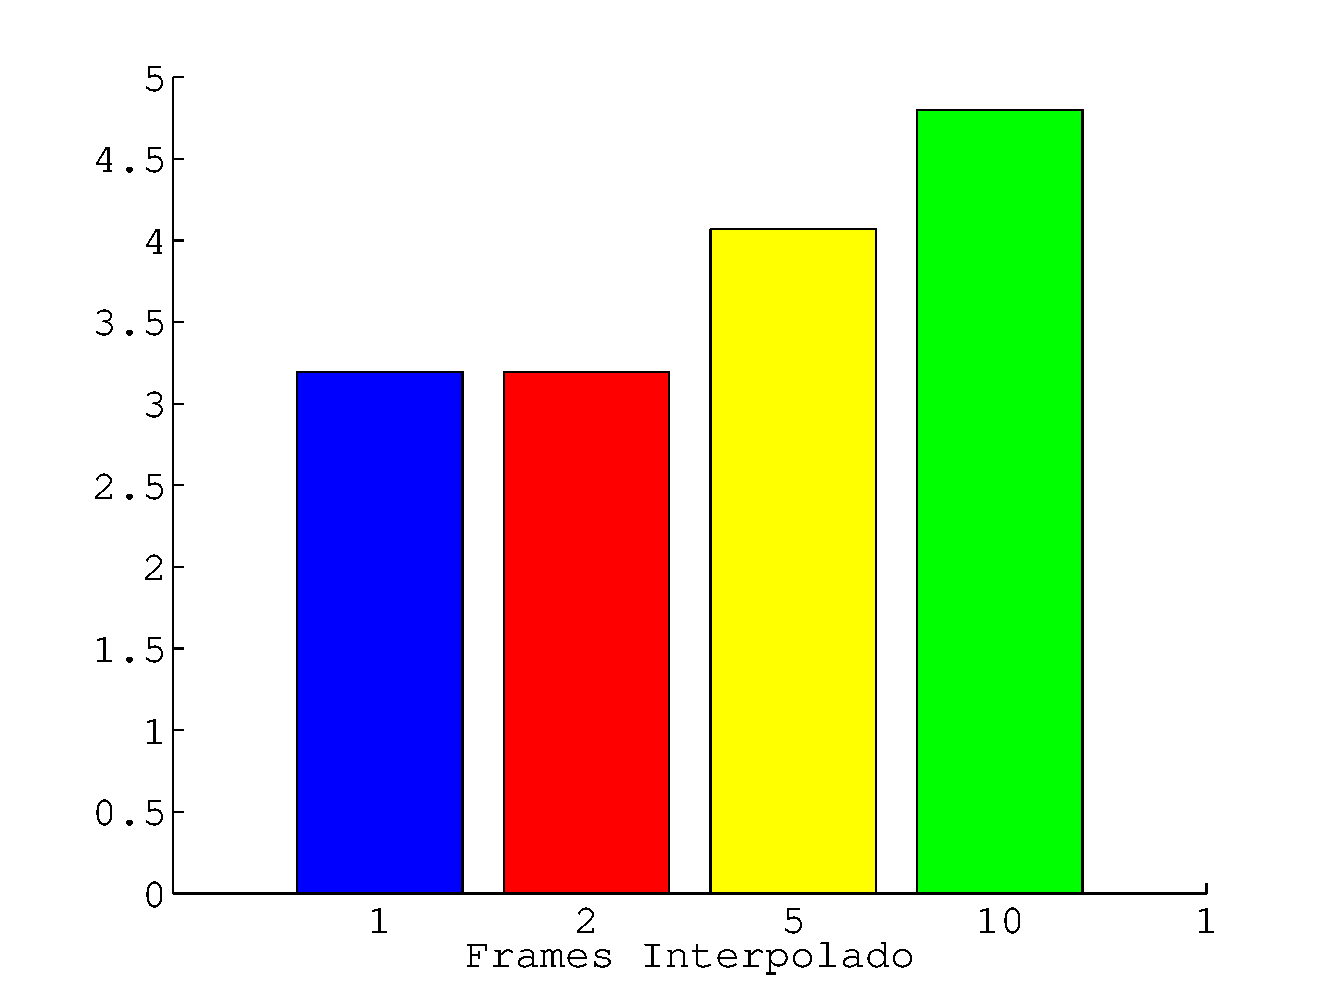
\includegraphics[width=.25\textwidth]{camara_fija-imagen_movil-mean_vecino.pdf}
    }
    \subfloat[][Desv\'io Est\'andar]{
        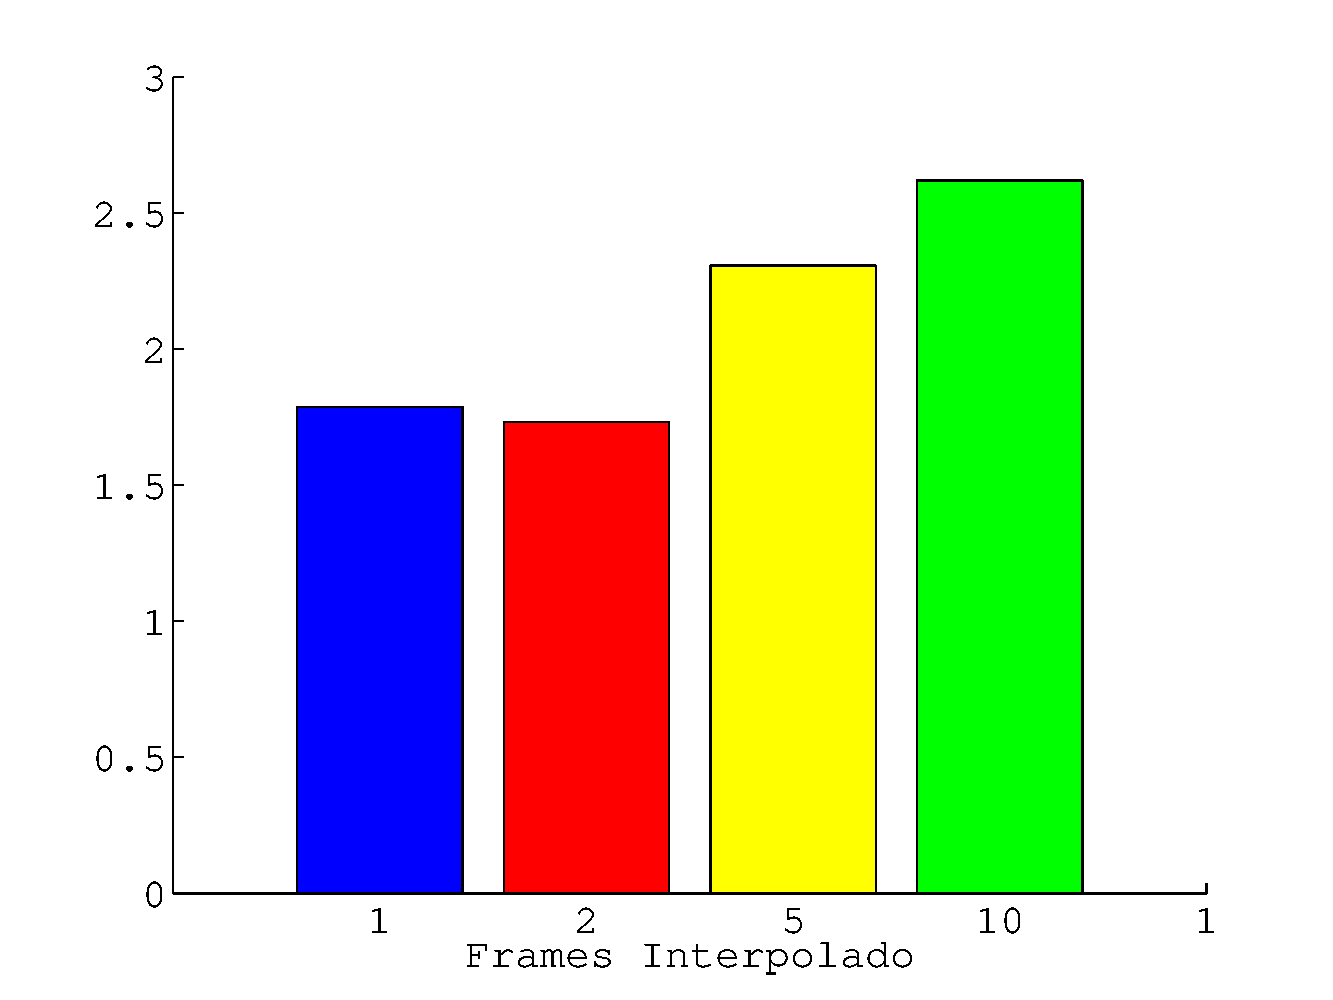
\includegraphics[width=.25\textwidth]{camara_fija-imagen_movil-std_vecino.pdf}
    }
    \subfloat[][M\'aximo]{
        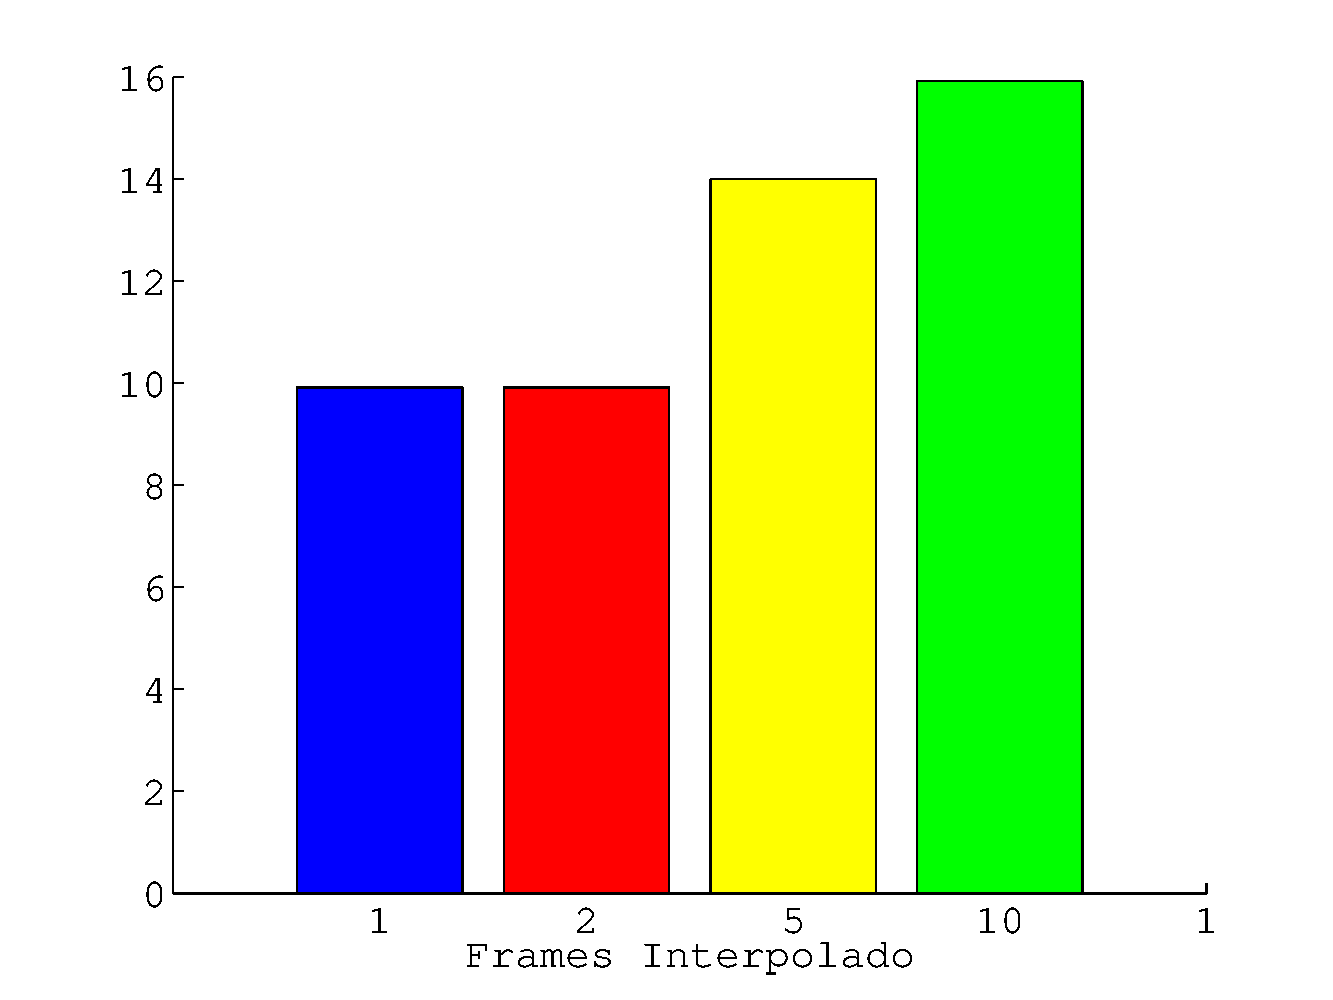
\includegraphics[width=.25\textwidth]{camara_fija-imagen_movil-max_vecino.pdf}
    }
    \subfloat[][M\'inimo]{
        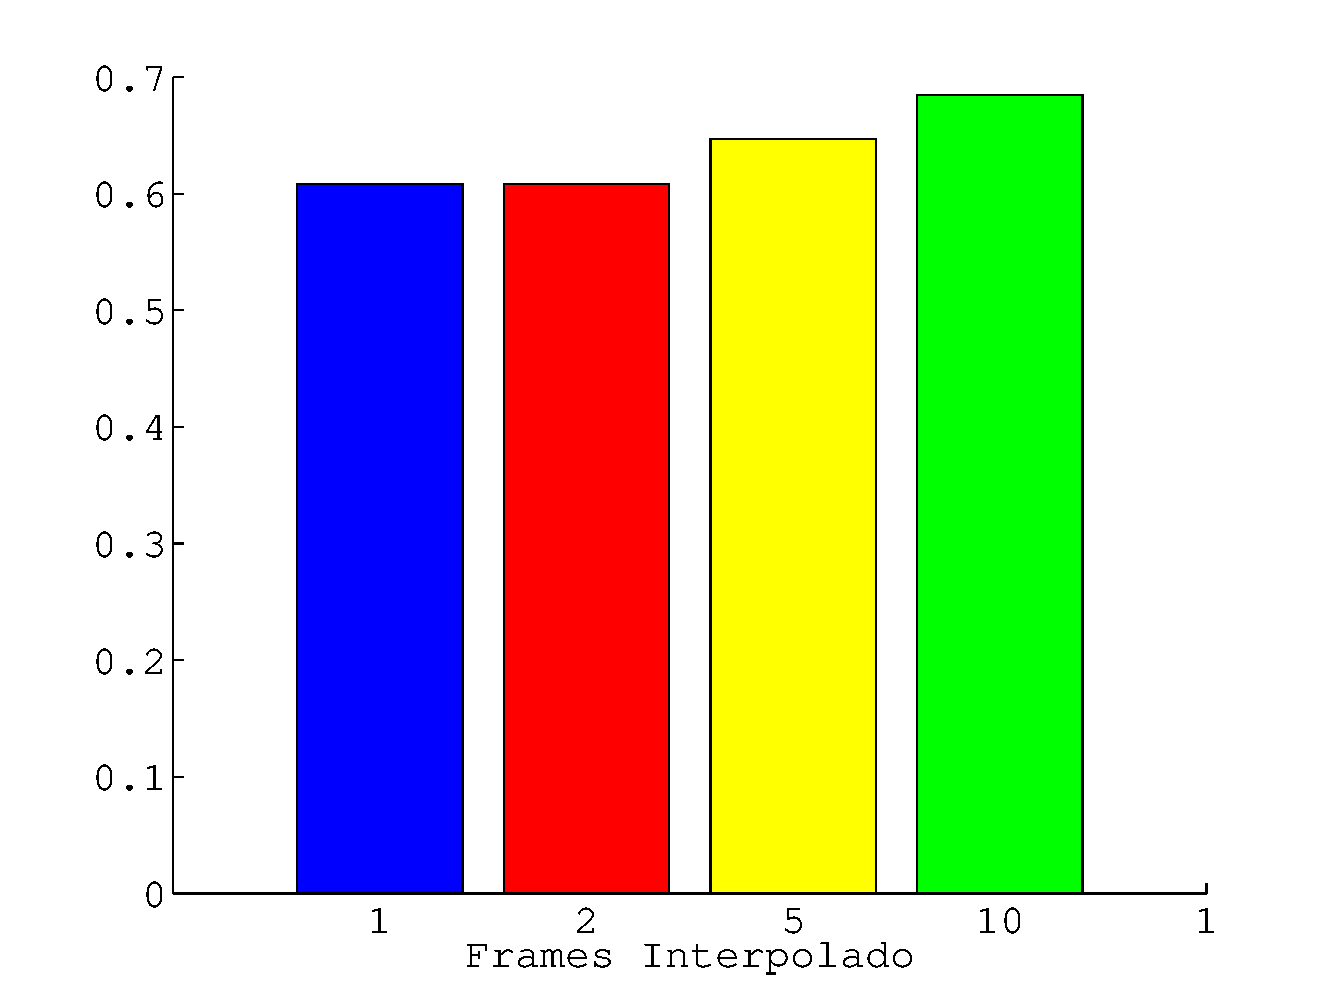
\includegraphics[width=.25\textwidth]{camara_fija-imagen_movil-min_vecino.pdf}
    }
    \caption{Est\'adisticas ECM Seg\'un Frames Interpolados - M\'etodo Vecino M\'as Cercano}
    \label{fig:fija-movil_vecino-mse_estadisticas}
\end{figure}

\par Nuevamente, para este m\'etodo y este video, encontramos resultados
consistentes con nuestras hip\'otesis. A mayor cantidad de frames interpolados,
mayor es el error medio. De hecho, los resultados de este m\'etodo son muy
similares a los de la interpolaci\'on lineal (en cuanto a la relaci\'on del
mismo m\'etodo para distintos frames interpolados, no en cuanto a los valores
de ECM de vecino m\'as cercano contra interpolaci\'on lineal). Aunque, salta a
la vista que el desv\'io est\'andar para la interpolaci\'on de 2 frames es
ligeramente menor que para la de 1 frame.

\par Voliendo sobre los conceptos del m\'etodo, es de alguna manera razonable
explicar esto debido a que al tener 2 frames interpolados por cada par
consecutivo de frames del video original, cada uno de los interpolados ser\'a
una copia exacta de su frame original m\'as cercano. De esta manera, deber\'ian
haber movimientos/cambios muy bruscos en los frames originales (como por
ejemplo, un cambio de c\'amara si se estuviera trabajando con el video de una
transimici\'on de televisi\'on o una pel\'icula) de manera que el frame
copiado/interpolado fuera completamente distinto al frame original al que
deber\'ia aproximar. Dado que esto no ocurre en nuestro video, es razonable
pensar que la diferencia de un frame a otro no tenga grandes diferencias, de
manera que al utilizar una copia del vecino m\'as cercano para una
interpolaci\'on de pocos frames no tenga demasiado error ni mucha varianza (ya
que el error de todos los frames interpolados/copiados es la diferencia de 2
frames consecutivos del video original, los cuales para un video sin cambios
bruscos deberia ser similar para todos los frames).

\par Analizando el video comparativo para este
m\'etodo\footnote{\url{https://drive.google.com/open?id=0B0RfkWV-4-XqY1gtZDFqQ0puaTg}},
adem\'as de observar el mismo comportamiento respecto de los movimientos/planos
donde se genera el error en la interpolaci\'on, observamos que hay saltos entre
frames donde el error aparece ''repentinamente''. Obviamente esto se debe a el
cambio de un frame a otro sin ning\'un intento de aproximar lo que ocurre en el
medio. Esto no ocurr\'ia para el experimento previo, ya que ahora tenemos
movimientos cuando antes s\'olo teniamos cambios de luz/tonalidad. Si bien no
podemos exponer en este documento en forma de gr\'afico esta percepci\'on, si
podemos presentar el gr\'afico del PSNR frame a frame, donde se puede observar
los picos de muy pronunciados de p\'erdida de precisi\'on (o aumento del error)
que ocurren de manera c\'iclica (con esto nos refer\'imos a que ocurren a un
intervalo regular de frames, no a que su valor PSNR sea el mismo).

\begin{figure}
    \centering
    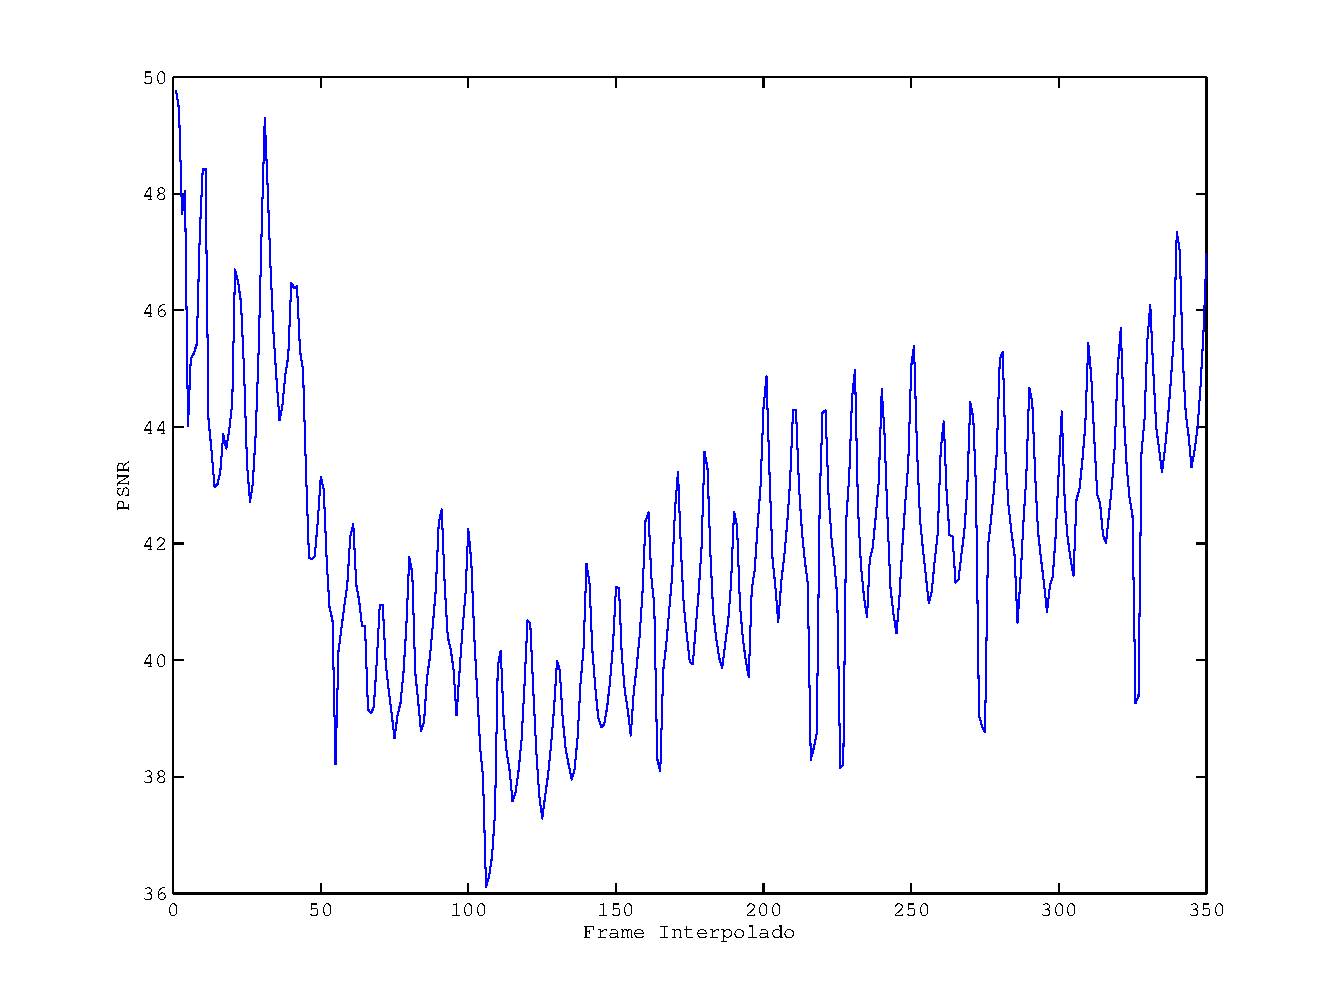
\includegraphics[width=.85\textwidth]{camara_fija-imagen_movil-vecino-psnr-k10.pdf}
    \caption{PSNR para 10 frames interpolados - Vecino m\'as Cercano}
    \label{fig:fija-movil_vecino-psnr-k10}
\end{figure}

\par Aqu\'i lo que se nota de distinto respecto de los otros m\'etodos, que por
ah\'i no es tanto el intervalo de los picos de error (bajo PSNR), es el hecho
de que los mismos son abruptos (pasan de un PSNR alto a un PSNR bajo de manera
muy r\'apida), mientras que en los casos anteriores observamos como estos cambios
se dan de forma m\'as ''suave'': es decir, graficamente hablando, de una manera
no tan ''recta'' sino m\'as curva (ver figura \ref{fig:fija-movil_lineal-psnr-k10}).

%---------------------------------------------------------------
\subsubsection{An\'alisis entre M\'etodos}

\begin{figure}[H]
    \centering
    \subfloat[][PSNR para 1 frames interpolados]{
        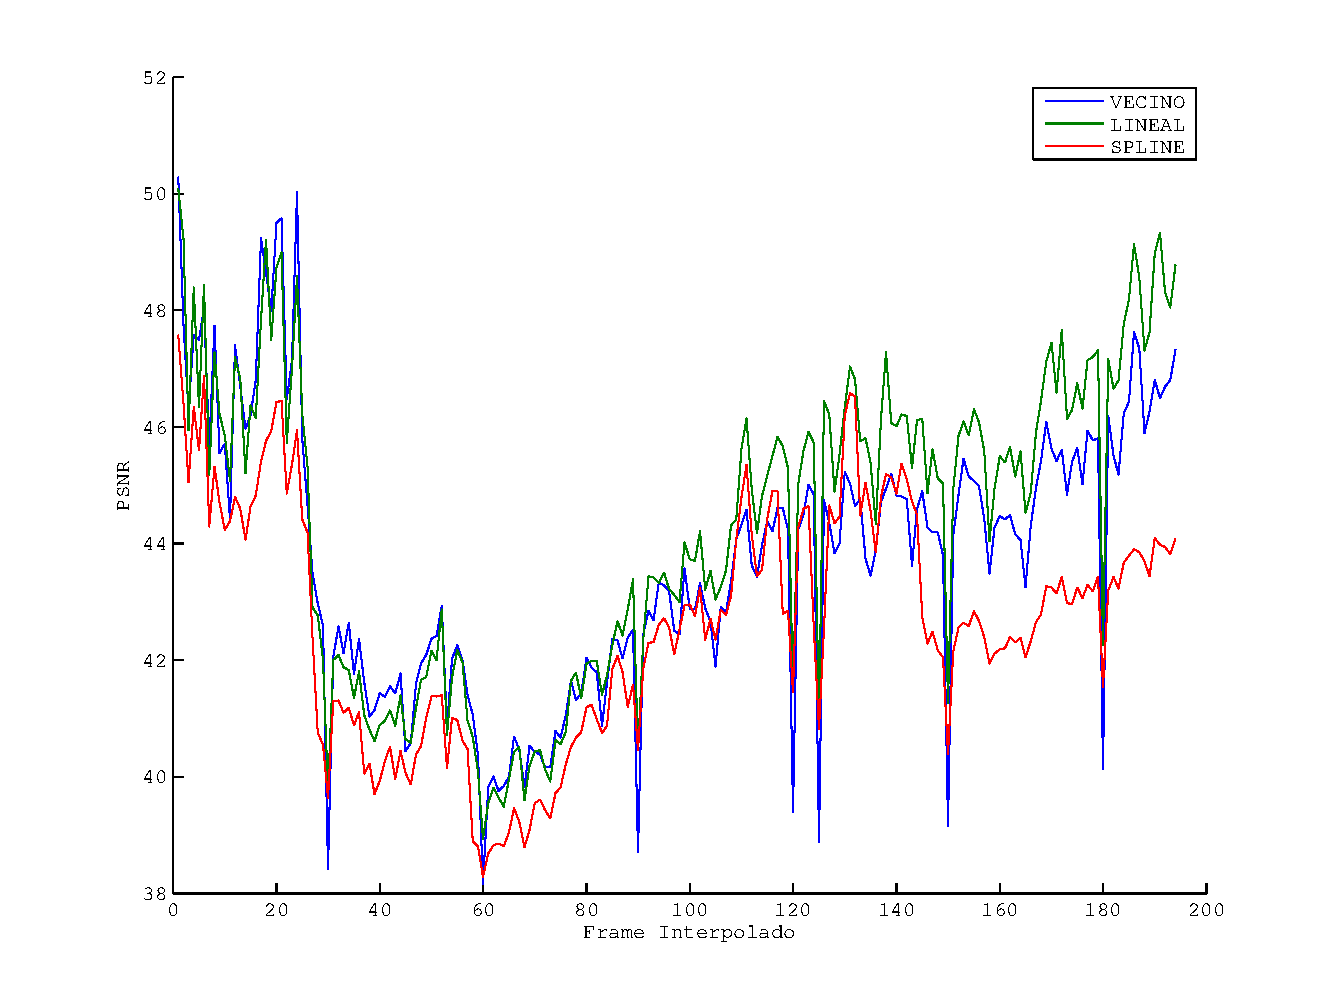
\includegraphics[width=.5\textwidth]{psnr_methods-camara_fija-imagen_movil-k1.pdf}
        \label{subfig:fija-movil_psnr-k1}
    }
    \subfloat[][PSNR para 2 frames interpolados]{
        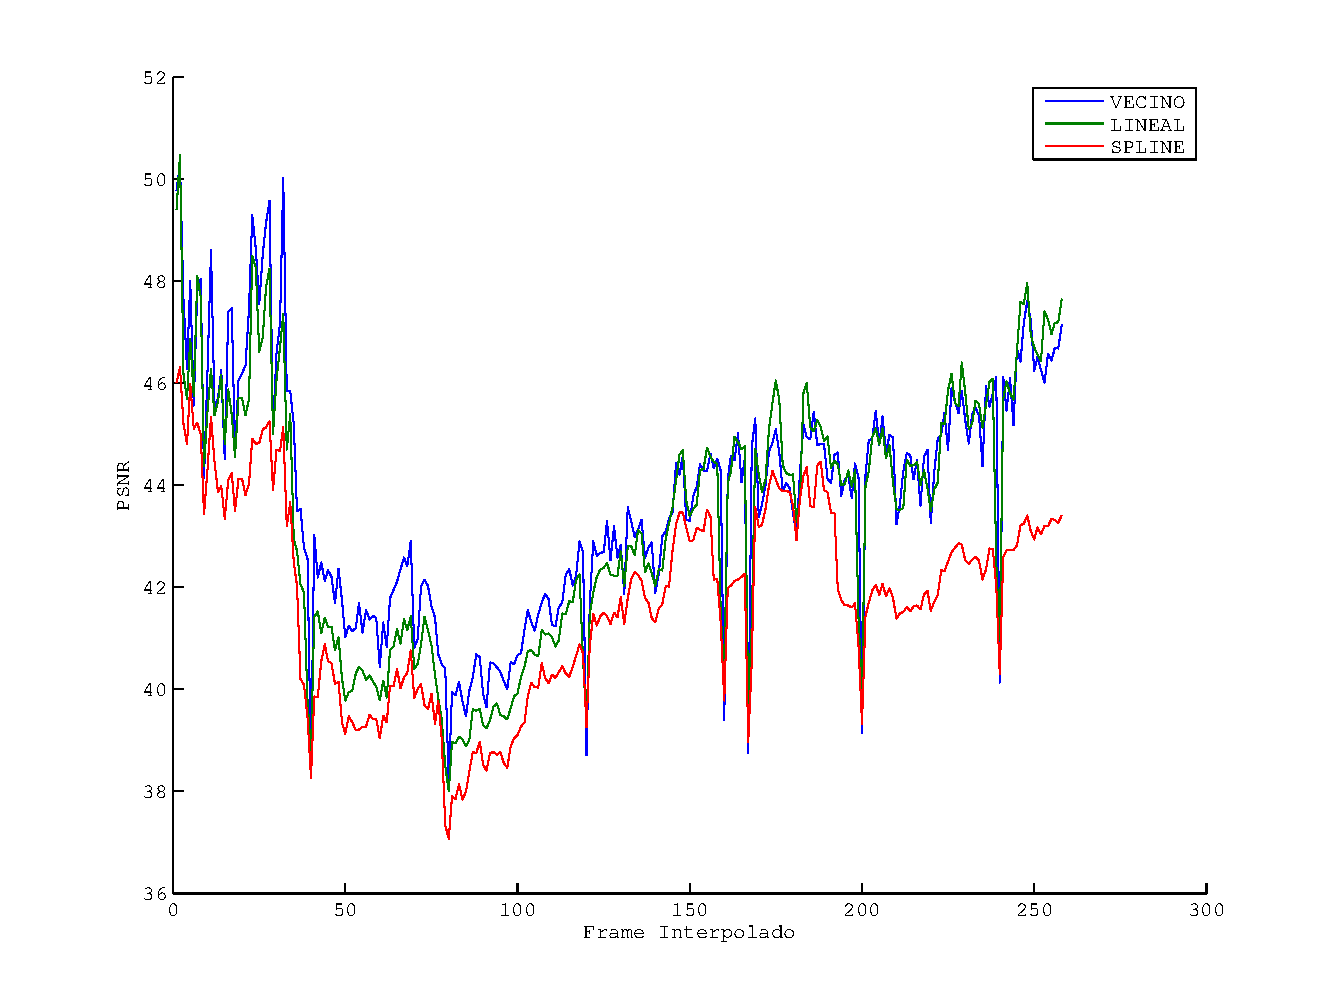
\includegraphics[width=.5\textwidth]{psnr_methods-camara_fija-imagen_movil-k2.pdf}
        \label{subfig:fija-movil_psnr-k2}
    }\\
    \subfloat[][PSNR para 5 frames interpolados]{
        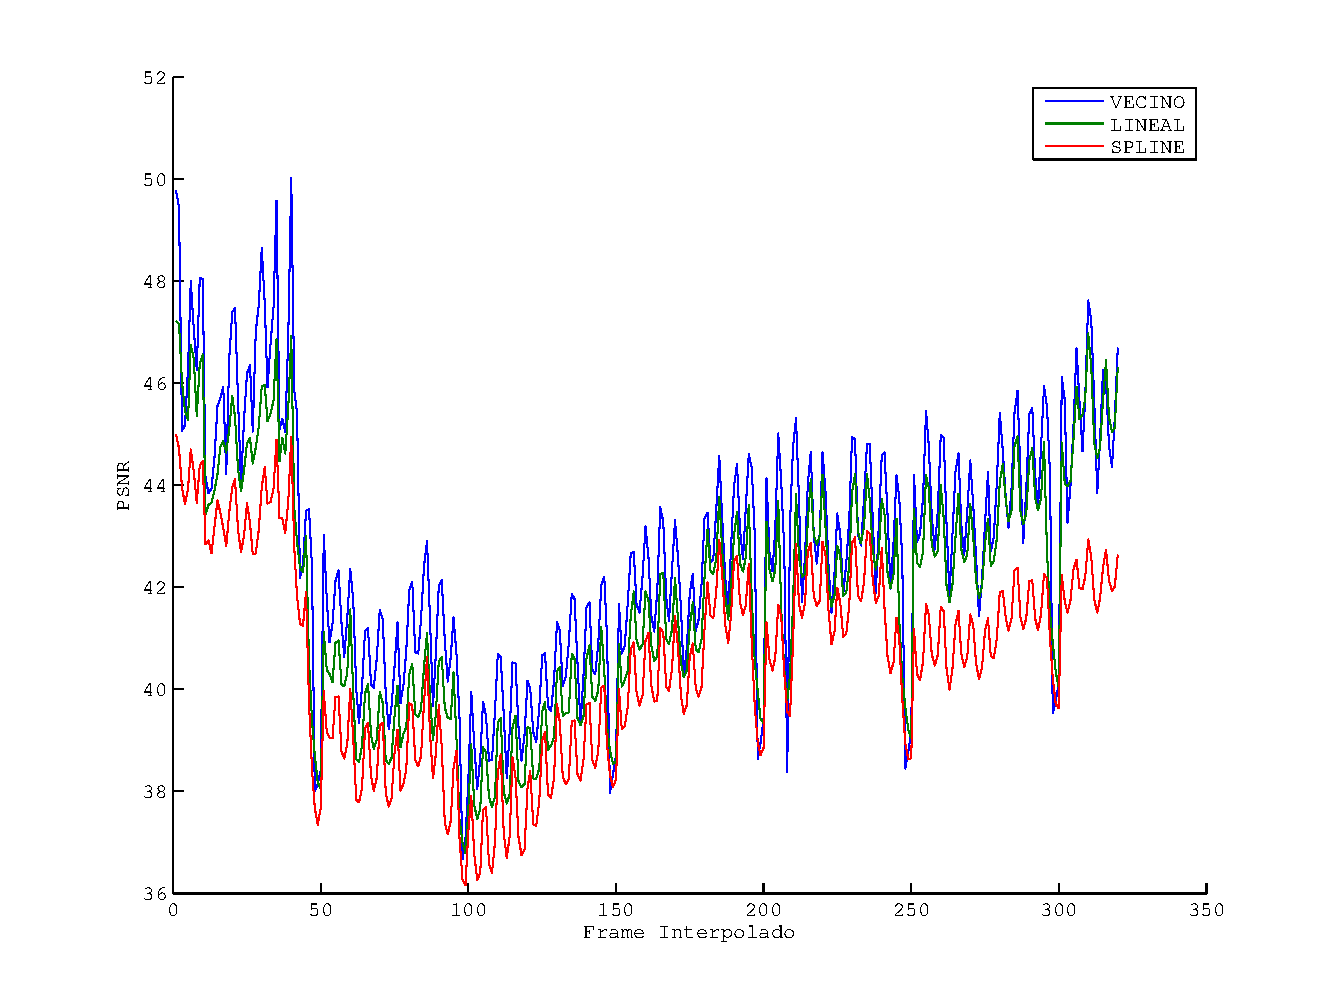
\includegraphics[width=.5\textwidth]{psnr_methods-camara_fija-imagen_movil-k5.pdf}
        \label{subfig:fija-movil_psnr-k5}
    }
    \subfloat[][PSNR para 10 frames interpolados]{
        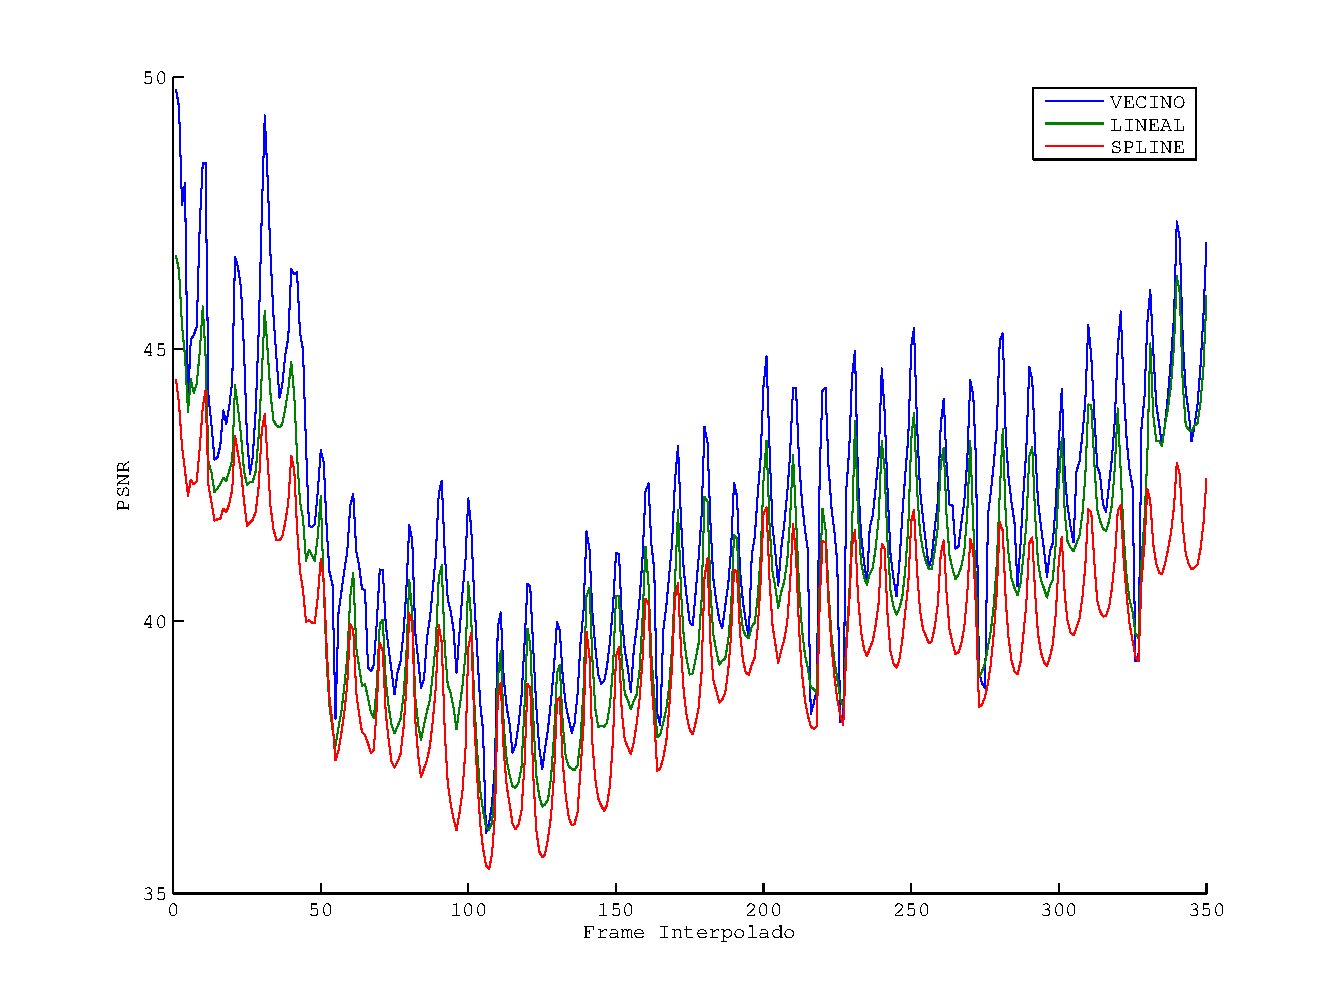
\includegraphics[width=.5\textwidth]{psnr_methods-camara_fija-imagen_movil-k10.pdf}
        \label{subfig:fija-movil_psnr-k10}
    }
    \caption{Comparativa de m\'etodos}
    \label{fig:fija-movil_metodos}
\end{figure}

\par En la figura \ref{fig:fija-movil_metodos} se presentan el PSNR para las
distintas variantes de cantidad de frames interpolados, comparando los m\'etodos
que objeto de estudio de este trabajo. En el caso particular del m\'etodo de
spline, se tom\'o el tama\~no de bloque 4, habi\'endose visto que este era el
que menor error presentaba para cualquiera de las variantes de cantidad de frames
interpodos.

\par Para todos las variantes expuestas, el primer resultado obvio es que
spline parecier\'a ser el m\'etodo que pero estima los frames. Se observa que
para todos los frames interpolados, es siempre el m\'etodo de menor PSNR. Y,
como ya se ha visto, splines es el m\'etodo m\'as costoso de los 3 que est\'an
siendo estudiados, con lo cual este resultado ya nos permite proponer que a la
hora de utilizar este tipo de videos (c\'amara fija, im\'agen m\'ovil -sin
movimientos bruscos-) splines no parece ser un m\'etodo a ser
considerado\footnote{Quiz\'as si evalu\'asemos variantes donde se interpolen
una mayor cantidad de frames, estos resultados podr\'ian variar. Pero ya tener
una interpolaci\'on de 10 frames es considerable, sumado las limitantes de
tiempo para experimentar con valores m\'as altos.}.

\par Queda entonces evaluar que ocurre con los m\'etodos del vecino e
interpolaci\'on lineal. Observando las figuras \ref{subfig:fija-movil_psnr-k1}
y \ref{subfig:fija-movil_psnr-k2}, se ve que en la primera mitad del video el
PSNR de ambos m\'etodos es similar, para luego en la segunda mitad obtener la
interpolaci\'on lineal mejores resultados (en el caso de 2 frames interpolados,
esta ventaja es m\'inima y quiz\'as desestimable). En los casos restantes, es
claro que durante todo el video el m\'etodo del vecino estima de mejor manera
los frames reconstru\'idos. No es casualidad que, en los casos donde la
interpolaci\'on lineal supera al m\'etodo del vecino, se de justo en el momento
en que aparece un jugador en el primer plano del video (alrededor del frame
110). Pareciera que al interpolar pocos frames y haber movimiento en un \'area
considerable de los frames el m\'etodo lineal se comporta mejor que el resto.
Lo sorpresivo es, dadas nuestras hip\'otesis, que al aumentar la cantidad de
frames el PSNR sea mucho mejor para el metodo del vecino.

\par Si observamos las estad\'isticas del ECM de la figura 
\ref{fig:fija-movil_methods-mse_estadisticas}, veremos que los resultados
reflejan este mismo comportamiento (bien podr\'ia, debido a un desv\'io est\'andar
alto o una cantidad de \emph{outliers} suficiente, no hacerlo). Se observa que
para pocos frames el ECM medio del m\'etdo lineal es menor, y que a medida que
aumenta la cantidad de frames estimados el m\'etodo del vecino comienza a tener
un ECM medio m\'as bajo relativo a los otros dos m\'etodos. Incluso esto mismo
ocurre con el desv\'io est\'andar (aunque la diferencia relativa que va ''ganando''
el m\'etodo del vecino crece a menor ratio).

\begin{figure}[H]
    \centering
    \subfloat[][Valor Medio]{
        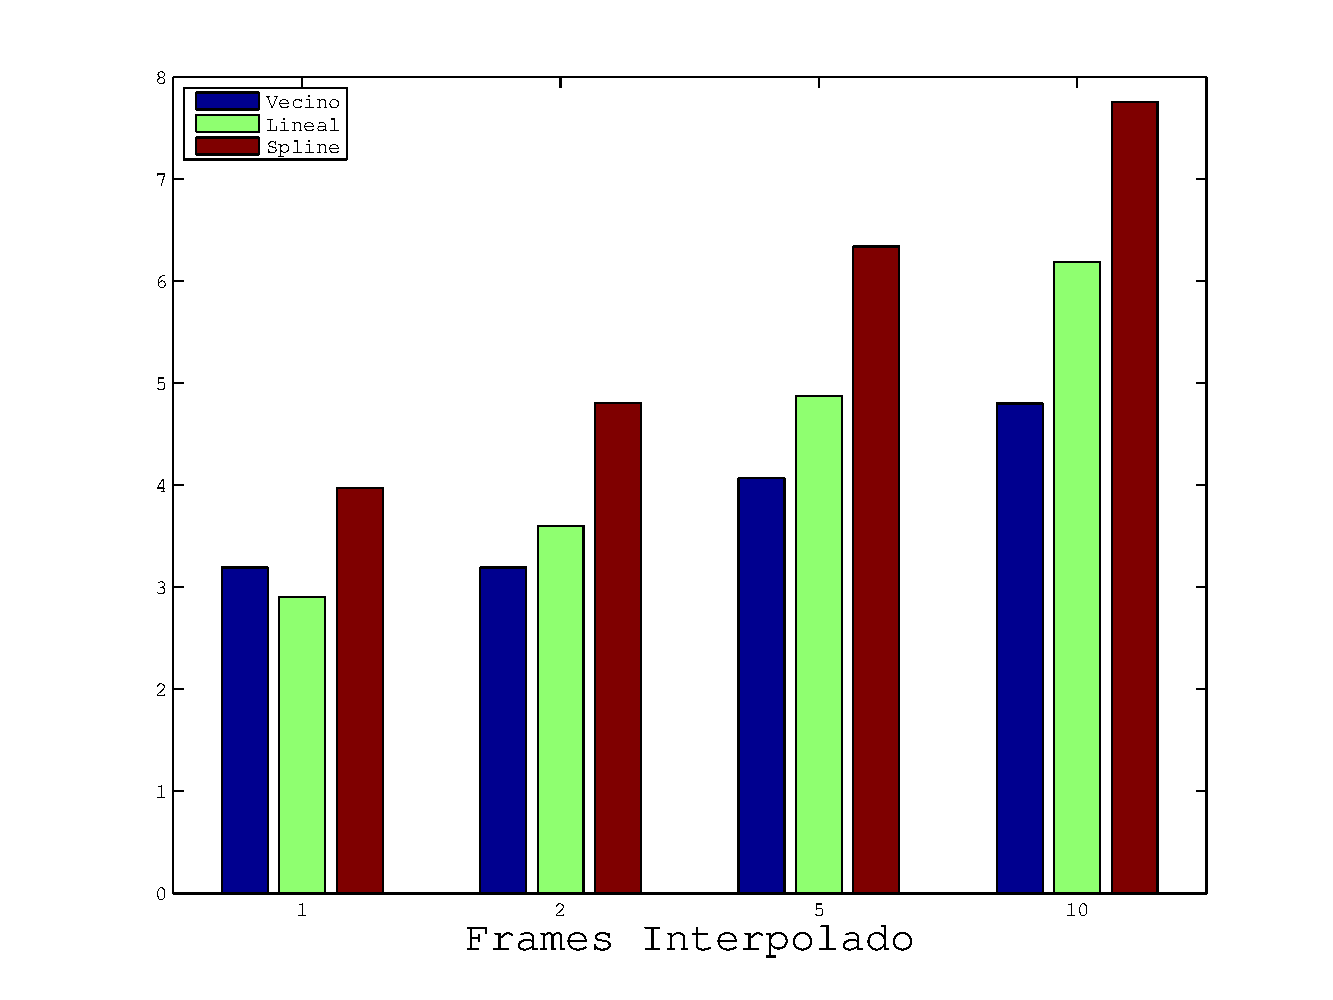
\includegraphics[width=.5\textwidth]{mean_methods-camara_fija-imagen_movil.pdf}
    }
    \subfloat[][Desv\'io Est\'andar]{
        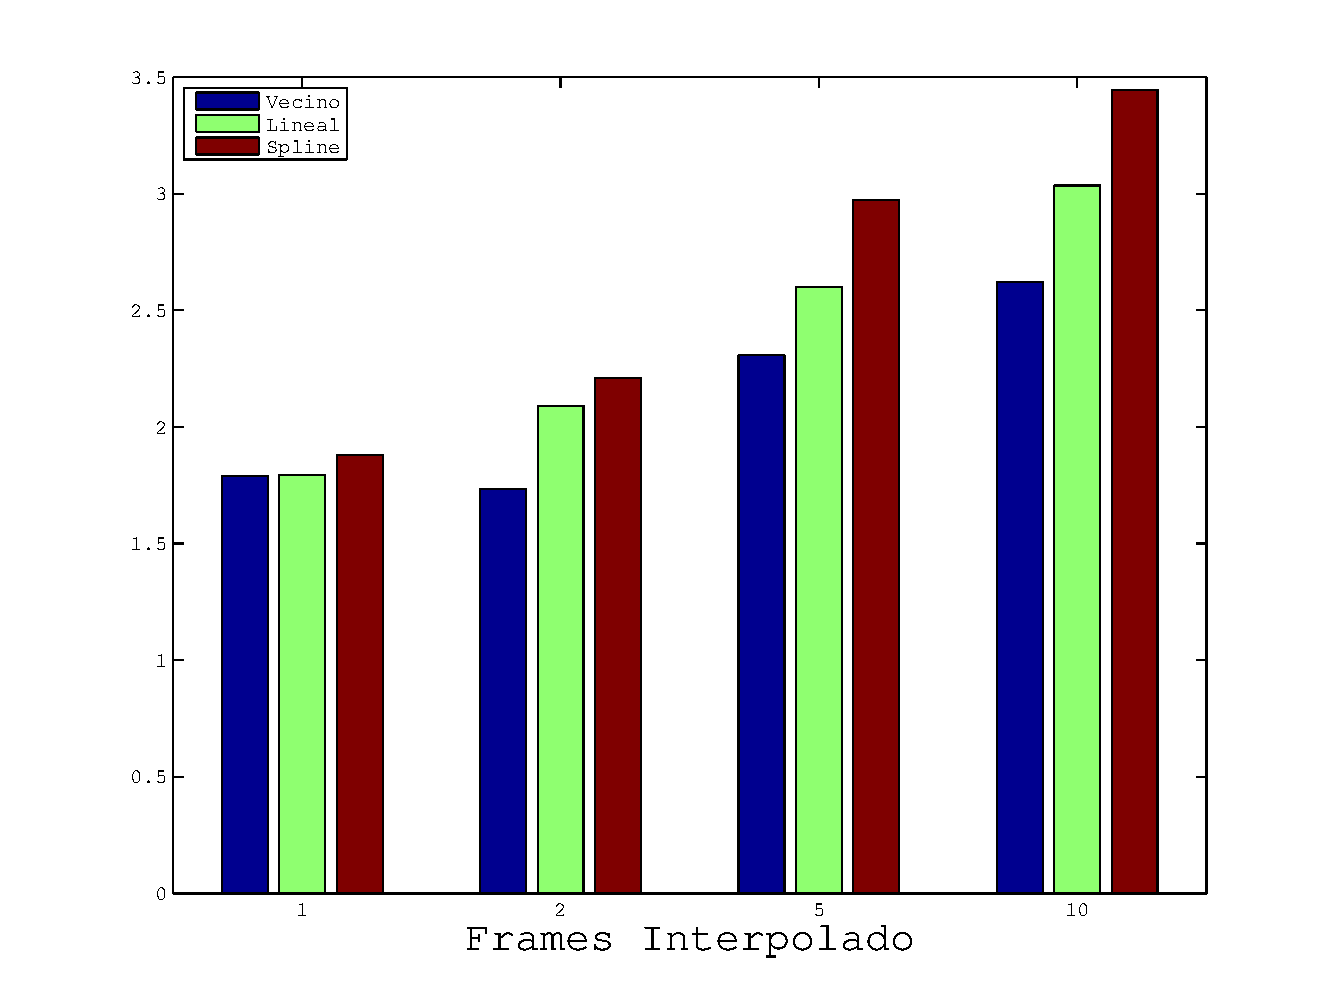
\includegraphics[width=.5\textwidth]{std_methods-camara_fija-imagen_movil.pdf}
    }\\
    \subfloat[][M\'aximo]{
        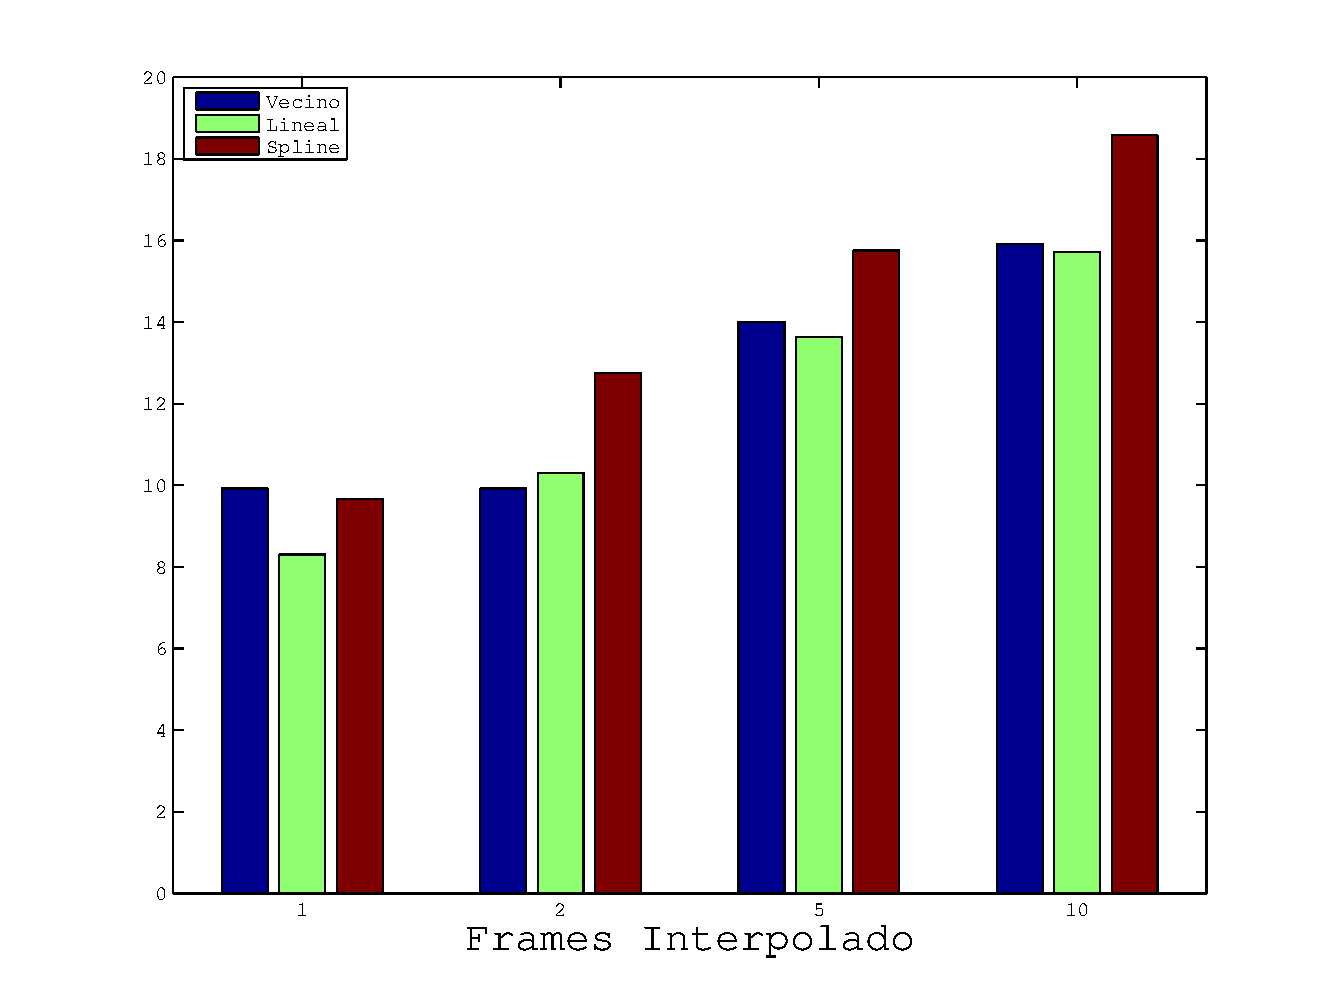
\includegraphics[width=.5\textwidth]{max_methods-camara_fija-imagen_movil.pdf}
    }
    \subfloat[][M\'inimo]{
        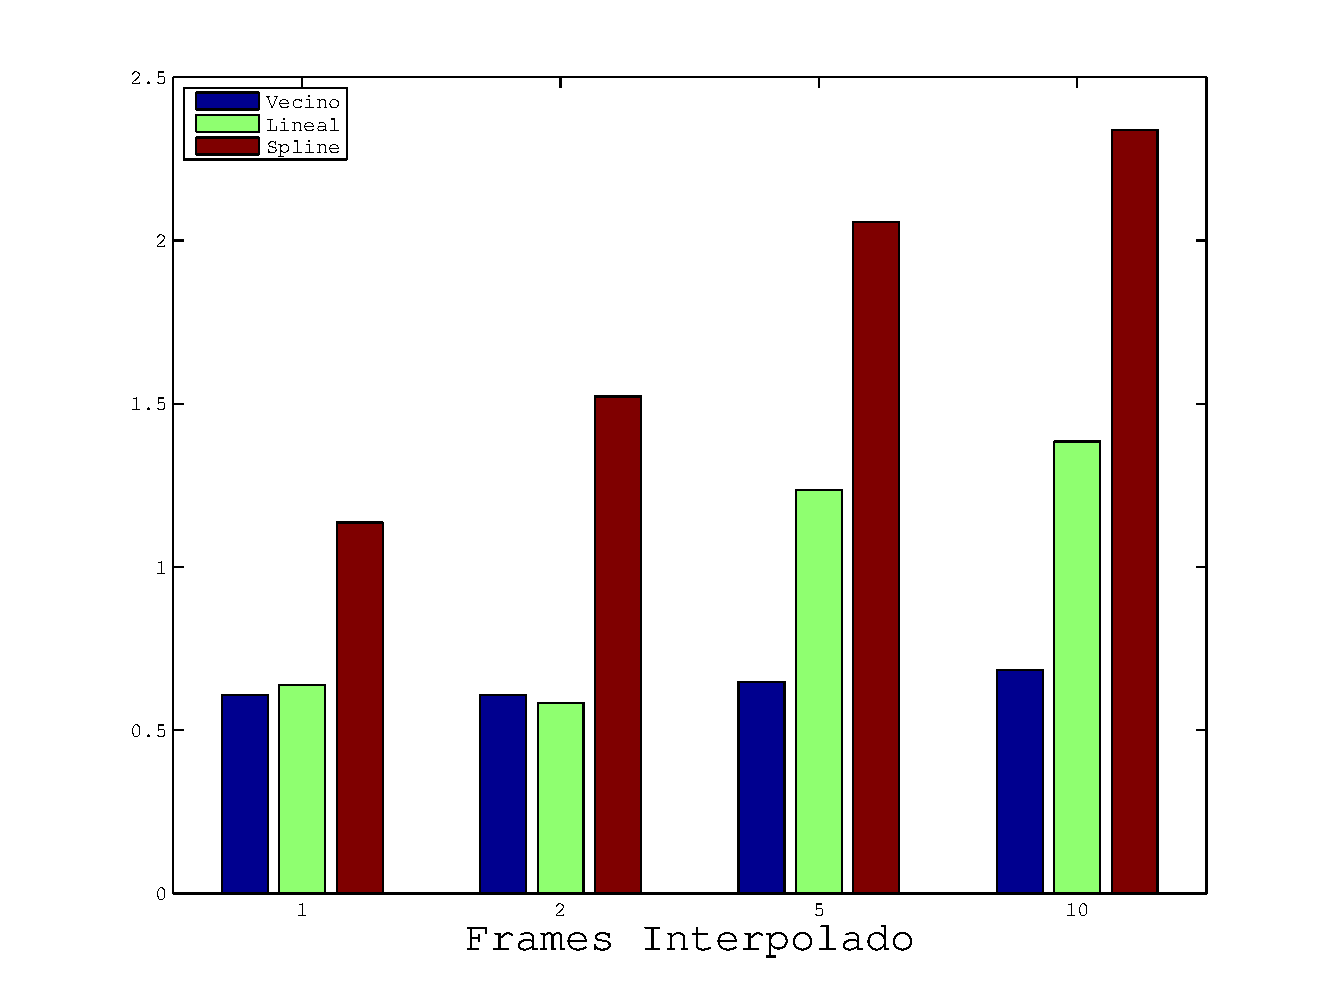
\includegraphics[width=.5\textwidth]{min_methods-camara_fija-imagen_movil.pdf}
    }
    \caption{Est\'adisticas ECM - Comparativa de M\'etodos}
    \label{fig:fija-movil_methods-mse_estadisticas}
\end{figure}

\par Continuando el an\'alisis de estos datos, se ve que el ECM m\'inimo para
el m\'etodo del vecino se ve casi inalterado sin importar la cantidad de frames
que se interpolen. Esto tiene sentido pues dado un frame, su frame interpolado
inmediato en la reproducci\'on ser\'a siempre el mismo sin importar cuantos
otros frames se copien hasta ''llegar'' al siguiente frame
no-interpolado/original. Por otro lado, si vemos que el comportamiento de los
m\'etodos restantes comienza cada vez a tener una peor cota para el frame mejor
aproximado a medida que se estima una mayor cantidad de frames. Claramente
estos m\'etodos son mucho m\'as sensibles a la ''distancia'' entre los frames
originales utilizados para calcular su polinomio interpolador\footnote{Recordar
que en nuestra experimentaci\'on se est\'a tomando un video y se le remueven
frames que luego ser\'an reconstru\'idos mediante los m\'etodos estudiados.}.

\par En cuanto al frame peor estimado (m\'aximo ECM) observamos que todas las
t\'ecnicas evaluadas comienzan a tener un frame cada vez peor aproximado. Esto,
de hecho, tiene sentido, ya que a medida que se incrementa la cantidad de
frames interpolados se deben generar artificialmente m\'as cuadros con menos
informaci\'on (frames originales m\'as ''distantes'' en la reproducci\'on del
video original). Claramente aproximar con menos informaci\'on reduce las
posibilidades de estimar de manera precisa.

\par Por \'ultimo, y para finalizar este an\'alisis de los m\'etodos para este
video, observamos los videos comparadores de utilizados en los an\'alisis
independientes de los m\'etodos para este video. A modo de presentar un resultado
en este trabajo, presentamos en la figura \ref{fig:fija-movil_heatmap} 3
capturas del mismo frame, que fue interpolado por los 3 m\'etodos.

\begin{figure}[H]
    \centering
    \subfloat[][Spline (tama\~no de bloque 4)]{
        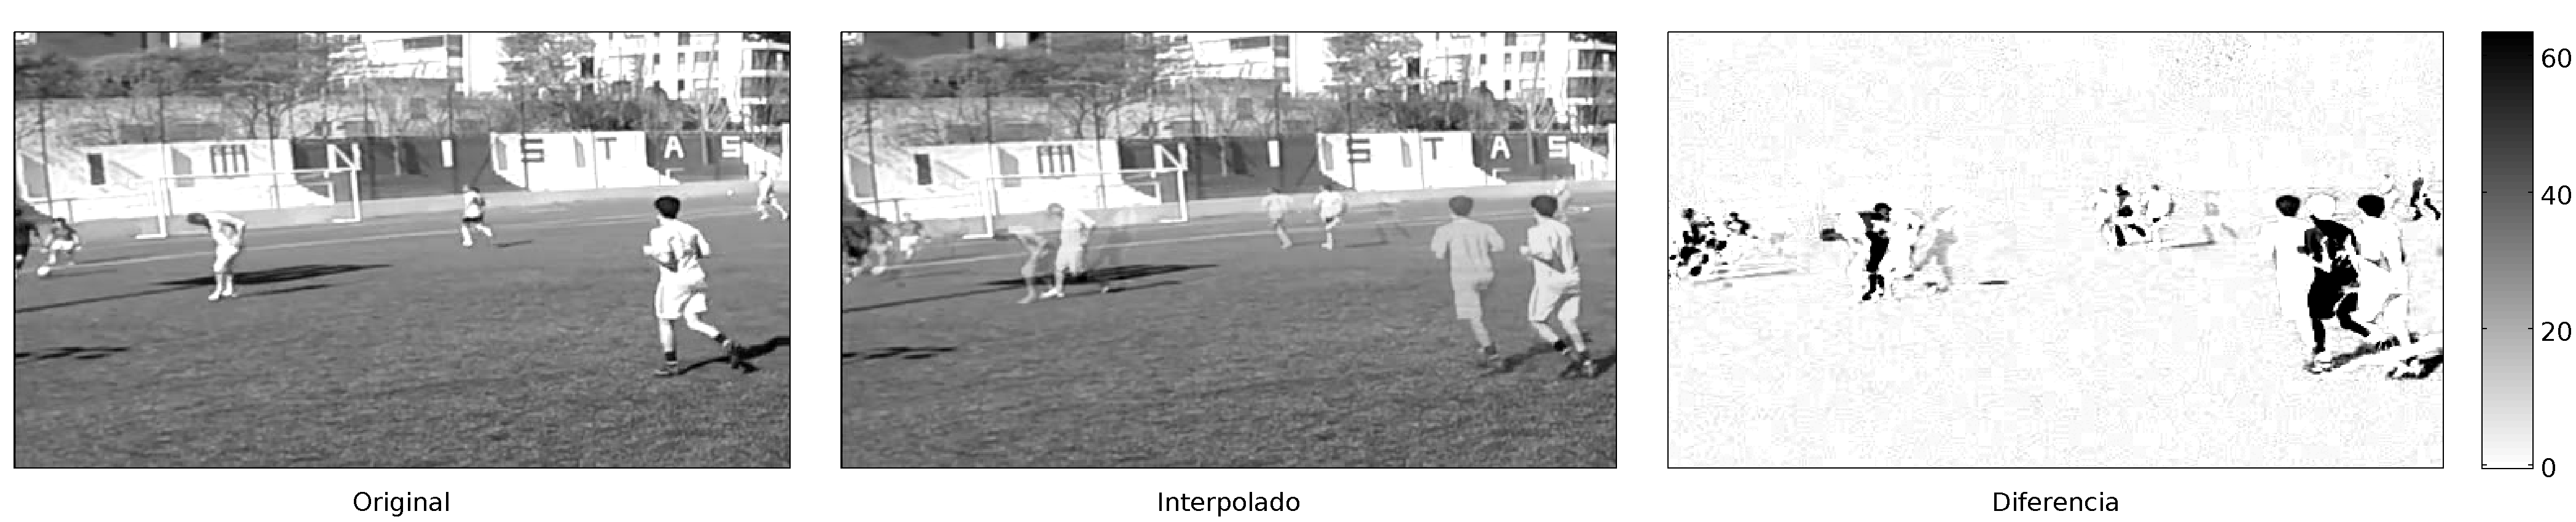
\includegraphics[width=\textwidth]{camara_fija-imagen_movil-spline-k10-blk4.png}
    }\\
    \subfloat[][Interpolaci\'on Lineal]{
        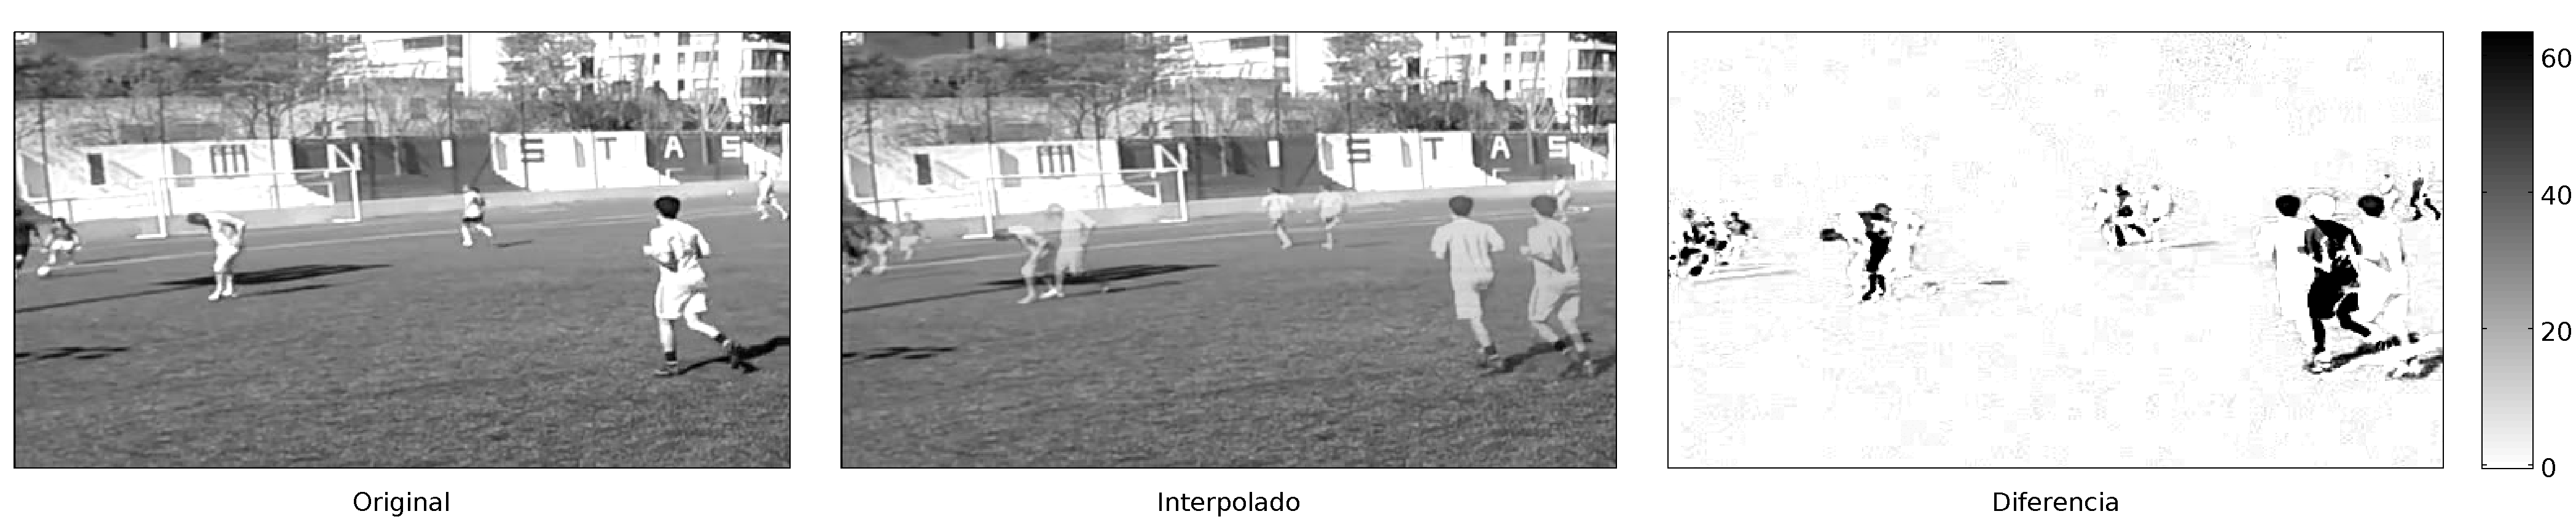
\includegraphics[width=\textwidth]{camara_fija-imagen_movil-lineal-k10.png}
    }\\
    \subfloat[][Vecino m\'as Cercano]{
        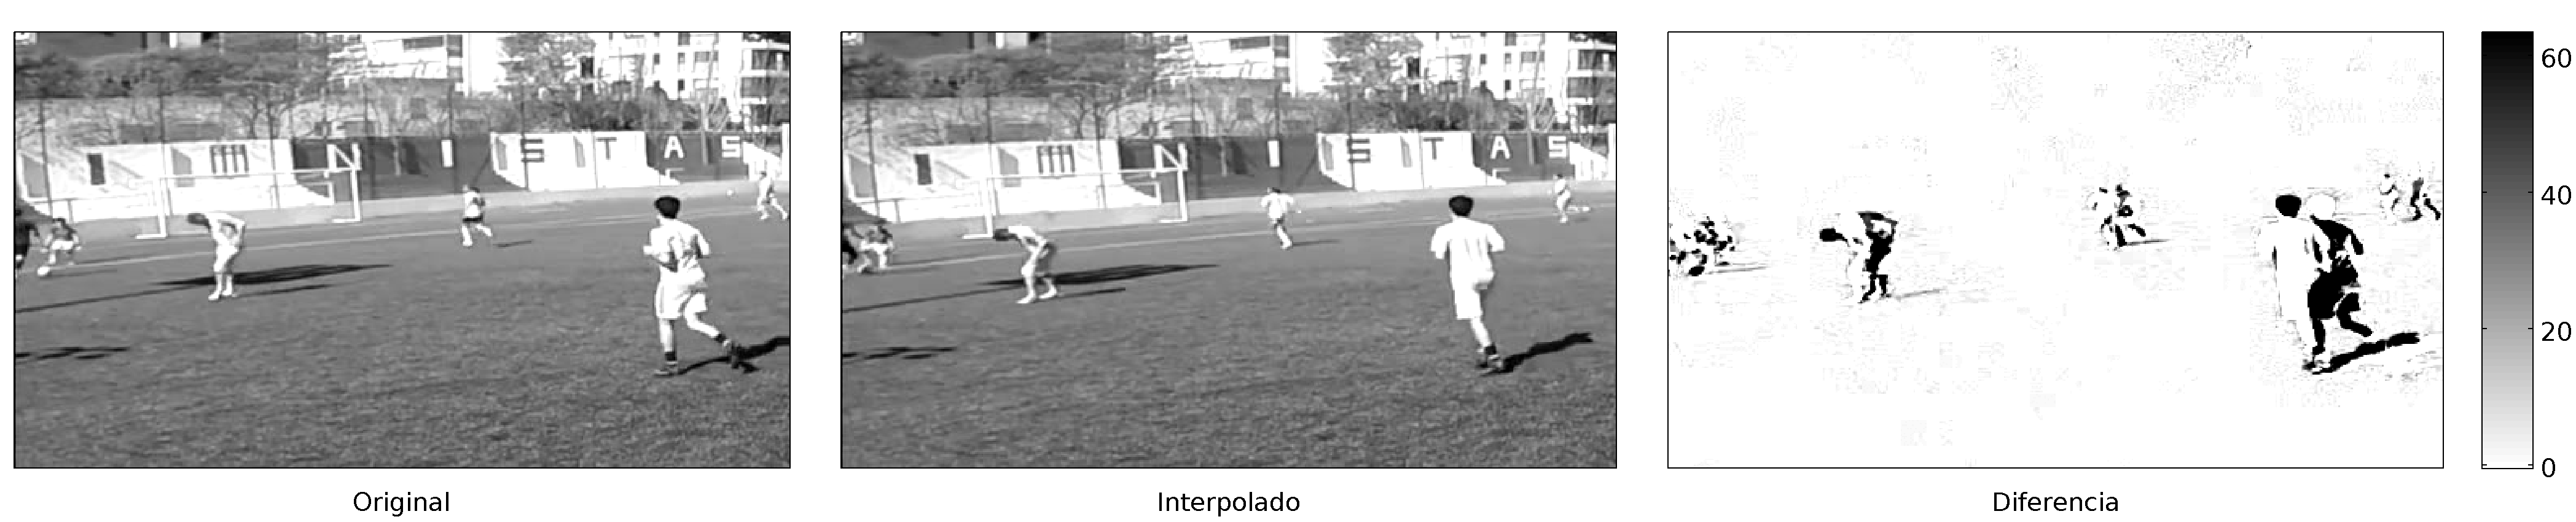
\includegraphics[width=\textwidth]{camara_fija-imagen_movil-vecino-k10.png}
    }
    \caption{Captura del mismo frame de Videos comparativos para interpolaci\'on de 10 frames}
    \label{fig:fija-movil_heatmap}
\end{figure}

\par Como se puede observar en las figuras (o en los videos, cuyos \emph{links}
pueden encontrarse en las secciones previas) se ve que el movimiento de los
jugarores es el principal \'area de los frames que son estimados de la manera
menos precisa por cualquiera de los m\'etodos. Lo intersante es obsevar las
\'areas de los frames que no presentan movimientos (o que son imperceptibles o
claramente de menor intensidad que los pertenecientes a los jugadores). As\'i
se puede observar que el m\'etodo de splines comete errores peque\~nos a lo largo
de todo el cuadro, mientras que el m\'etodo lineal lo hace en menor medida y el
vecino m\'as cercano a\'un menos.

\par Esto nos explica, probablemente, porque el m\'etodo del vecino tiene un
ECM menor que los otros dos m\'etodos (o PSNR m\'as alto). Observando las tonalidades
de los errores de los jugadores, y el \'area que ocupan en el frame estos puntos
\textbf{negros}, observamos que los m\'etodos cometen errores similares a la hora
de estimar a los mismos. Por lo tanto, queda claro que es la estimaci\'on del
resto del frame que hace que un m\'etodo tenga menor error que otro.

\par El porque de este comportamiento podr\'ia explicarse dado que el m\'etodo
del vecino es m\'as ''bobo'' (aunque en este caso pareciera ser una ventaja), ya
que no asume nada sobre los pixeles y solo los copia. De esta manera, al tener
una gran parte de los cuadros del video que son est\'aticos (o con poqu\'isimo
movimiento) y no llegan a tener cambios de iluminaci\'on (como en el caso del
experimento previo), logra replicar este estatismo. Los m\'etodos restantes
tratan a cada pixel como una funci\'on a ser interpolada, con lo cual asumen
que entre pixel y pixel siempre habr\'a alg\'un cambio (salvo que todos los
pixeles utilizados para calcular el polinomio interpolador tengan el mismo valor,
en cuyo caso el polinomio resultante corresponde a una funci\'on constante, pero
como en el video estos p\'ixeles sufren cambios muy peque\~nos esto no ocurre).

%---------------------------------------------------------------
\subsubsection{Conclusiones}
\par A lo largo de este experimento se ha visto, nuevamente, un patr\'on de
comportamiento para el m\'etodo de spline seg\'un su tama\~no de bloque. A
diferencia del experimento previo donde se vi\'o que el tama\~no parec\'ia no
afectar a la precisi\'on de la estimaci\'on, se observ\'o que en el caso de
este video un tama\~no peque\~no de bloque resulta m\'as efectivo.

\par Sorprendente es el resultado de que el m\'etodo del vecino m\'as cercano
estima de mejor manera que sus alternativas (salvo en el caso de pocos frames
interpolados, en cuyo caso el m\'etodo de interpolaci\'on lineal podr\'ia llegar
a ser mejor, dependiendo de las caracter\'isticas del video). M\'as interesante
a\'un es que este comportamiento pudo ser explicado, y es razonable aunque no
sea (al menos para los autores) intuitivo.

\par Ahora bien, habiendo comparado los m\'etodos mediante las m\'etricas y
conclu\'ido que m\'etodo resulta mejor para este tipo de casos, queda decir
si esto coincide con la percepci\'on subjetiva de quienes observan el video
interpolado. Y es aqu\'i donde los resultados obtenidos a partir de las m\'etricas
no se condicen con la percepci\'on humana\footnote{S\'i, somos humanos los
estudiantes de exactas.}.

\par Es la opini\'on de los autores que el m\'etodo del vecino consigue mejores
resultados en el caso de interpolar 1 o 2 frames. Pero en el caso de interpolar
10 frames, consideran que el m\'etodo del vecino es claramente el que peor
logra aproximar al video original Esto mismo se da ya que al ver el video, el
mismo pareciera tener alg\'un tipo de error de reproducci\'on o \emph{freeze},
debido a que se queda ''congelado'' en varios cuadros y da la sensaci\'on de
que muchos cuadros no se llegan a reproducir por alg\'un tipo de problema (que
no existe, ya que lo que ocurres es que se est\'a reproduciendo el mismo frame
unas 5 veces, ya que el m\'etodo copio el mismo). En este caso, la percepci\'on
del m\'etodo lineal o de splines es similar, con lo cual a la hora de elegir se
sugerir\'ia elegir el m\'etodo de interpolaci\'on lineal ya que es menos
costoso que splines, en cu\'anto al tiempo de c\'omputo requerido para
procesarlo.

\par As\'i pues, se ha llegado a un caso donde los resultados de laboratorio
basados en m\'etricas objetivas se contraponen con la percepci\'on de los
espectadores. Claramente los videos tienen otras variables que hacen a la
percepci\'on humana que nuestras m\'etricas no logran reflejar, justificando
para futuros trabajos la b\'usqueda de m\'etricas o variables que puedan modelar
esta percepci\'on subjetiva.

%---------------------------------------------------------------
